\documentclass[conference]{IEEEtran}
\IEEEoverridecommandlockouts

\usepackage{cite}
\usepackage{amsmath,amssymb,amsfonts}
\usepackage{algorithm}
\usepackage{algpseudocode}
\usepackage{graphicx}
\usepackage{booktabs}
\usepackage{textcomp}
\usepackage{xcolor}
\usepackage{url}
\usepackage{hyperref}
\usepackage{caption}
\usepackage{float}
\usepackage{microtype}
\usepackage{array}

\hypersetup{colorlinks=true, linkcolor=blue!50!black,
            citecolor=blue!50!black, urlcolor=blue!60!black,
            pdftitle={Predicting Buchwald-Hartwig C-N Coupling Reaction Success},
            pdfauthor={Gurpreet Singh and Md Rafi}}

\graphicspath{{figures/report/}}

\def\BibTeX{{\rm B\kern-.05em{\sc i\kern-.025em b}\kern-.08em
    T\kern-.1667em\lower.7ex\hbox{E}\kern-.125emX}}

\begin{document}

\title{Predicting Buchwald--Hartwig C--N Coupling Reaction Success:\\
       From Yield Regression to Binary Triage with\\
       $k$-Way Combinatorial Fusion Analysis}

\author{\IEEEauthorblockN{Gurpreet Singh}
\IEEEauthorblockA{\textit{Department of Computer Science} \\
\textit{Fordham University}\\
New York, NY, USA \\
gsingh60@fordham.edu}
\and
\IEEEauthorblockN{Md Rafi}
\IEEEauthorblockA{\textit{Department of Computer Science} \\
\textit{Fordham University}\\
New York, NY, USA \\
mrafi2@fordham.edu}}

\maketitle

\begin{abstract}
Predicting the yield of palladium-catalysed C--N cross-coupling reactions is
a long-standing problem in pharmaceutical synthesis: a Buchwald--Hartwig
amination appears in the route to a large fraction of approved
small-molecule drugs, and unsuccessful attempts cost weeks of bench time and
substantial reagent cost. We present a two-stage study on $5{,}465$
Buchwald--Hartwig reactions extracted from the Open Reaction Database. In
stage one we trained a pool of $41$ regression models---linear, kernel,
tree-ensemble, gradient-boosting, neural and chemistry-aware (Chemprop
D-MPNN, NGBoost, rxnfp+LightGBM, Gaussian process with Tanimoto kernel)---on
$\sim$$14{,}337$-dimensional fingerprint features and combined them with
$k$-way \emph{Combinatorial Fusion Analysis}~(CFA). On a random $70/15/15$
split the best CFA ensemble reaches $R^{2}=0.836$, exceeding published
DRFP+XGBoost on comparably diverse data, but on a scaffold-based
out-of-distribution split \emph{every} regressor collapses to negative test
$R^{2}$, a known consequence of reporter bias and scaffold--yield coupling
in literature reaction databases. In stage two we pivot the task: instead of
predicting an absolute yield number we predict whether the reaction will
exceed a chemistry-relevant \emph{success threshold} of $50\%$ yield, the
binary go/no-go decision a synthetic chemist actually makes. The classifier
reaches $92.4\%$ accuracy, MCC $+0.83$, AUC $0.97$, Brier $0.045$ on a
random split, $82\%\pm5\%$ accuracy on substrate-grouped 5-fold CV, and
recovers above-baseline accuracy ($59.1\%$, MCC $+0.18$, AUC $0.64$) on
unseen Murcko scaffolds---where regression was unusable. A multi-seed
($n\!=\!10$ paired cells) Wilcoxon analysis modelled on the companion
quantum--classical CFA pipeline of
Patten~\textit{et al.}~\cite{Patten2026Quantum} confirms the
fused-vs-best-individual lift across both splits. We release code,
trained model artefacts, a CD-kneedle-based finalist-selection variant
of $k$-way CFA, and a calibrated Streamlit triage tool with a
reject-option wrapper for model disagreement.
\end{abstract}

\begin{IEEEkeywords}
Reaction yield prediction, Buchwald--Hartwig amination, combinatorial fusion
analysis, ensemble learning, message-passing neural networks, scaffold
out-of-distribution generalisation, cheminformatics, machine learning for
chemistry.
\end{IEEEkeywords}

% ============================================================================
\section{Introduction}
\label{sec:intro}

Carbon--nitrogen (C--N) bond formation through palladium-catalysed
Buchwald--Hartwig amination~\cite{Wolfe1996,Hartwig1998} is among the most
heavily used transformations in modern medicinal chemistry: a recent industry
analysis reports that an aryl C--N bond appears in over $80\%$ of FDA-approved
small-molecule drugs containing aromatic nitrogen, and the Buchwald--Hartwig
reaction is the dominant single retrosynthetic disconnection used to install
it~\cite{Schneider2016}. Despite four decades of mechanistic refinement,
\emph{a priori} prediction of yield for a previously unattempted substrate
pair remains unreliable: outcomes depend on a combinatorial interaction of
substrate electronics, ligand bulk, base strength, solvent polarity and
temperature, and are sensitive to the choice of any one
component~\cite{Buitrago2018}.

A reliable yield model would compress an otherwise multi-week experimental
screen---typically tens to hundreds of high-throughput experimentation~(HTE)
wells per substrate pair---to a ranked computational shortlist, deferring
bench time only to the most promising conditions. Two of the most widely
cited successes are the high-throughput Buchwald--Hartwig dataset of
Ahneman~\textit{et al.}~\cite{Ahneman2018} (random forest with DFT
descriptors, $R^{2}=0.92$ on a controlled $4{,}608$-reaction screen) and the
\emph{Yield-BERT} reaction transformer of
Schwaller~\textit{et al.}~\cite{Schwaller2021YB} ($R^{2}=0.951$ on the same
data). Performance reported on the Ahneman corpus, however, is well known to
overestimate real-world performance: the Ahneman dataset varies only four
reagent classes around a single solvent--temperature point, while real
laboratory notebook (ELN) yields recorded with full chemical heterogeneity
collapse those same models to $R^{2}\approx 0$~\cite{Fitzner2023,Wigh2024,Saebi2023}.

In this work we take the harder route. We extract $5{,}465$ Buchwald--Hartwig
reactions from the Open Reaction Database~(ORD)~\cite{Kearnes2021}, where
solvent, ligand and temperature vary freely; we train a $41$-model regression
pool on a shared $\sim$$14$k-dimensional fingerprint feature; we combine the
predictions with $k$-way Combinatorial Fusion Analysis (CFA), extending the
classical pairwise framework of Lin~\textit{et al.}~\cite{Lin2007} to
$k=2,\dots,5$; we replicate the in-distribution performance reported by the
literature; and we then \emph{deliberately fail} on a scaffold-OOD split to
expose the reporter-bias problem. We finish by reframing the task to binary
success classification at the chemically meaningful $50\%$ yield threshold,
recovering deployable performance without retraining a single regressor.

\medskip
\noindent\textbf{Contributions.}
\begin{itemize}
\item A pipeline that handles $41$ heterogeneous regressors over a shared
      $\sim$$14{,}337$-dimensional Morgan/DRFP feature vector without
      per-model reimplementation.
\item A regression-form $k$-way CFA implementation that calibrates the
      $[0,1]$-normalised combined score back onto the yield scale via
      least-squares fit on the validation set, so the resulting $R^{2}$ is
      directly comparable to single-model $R^{2}$.
\item A classification-form CFA reversion (eligibility filter
      $\mathrm{MCC}>0$, val-optimal threshold per ensemble) that reuses the
      same $41$ regressors as score generators without retraining.
\item Empirical confirmation that scaffold-OOD regression failure cannot be
      salvaged by ensemble diversity: every $k\in\{1,\dots,5\}$ ensemble
      collapses below $R^{2}=0$ on unseen scaffolds.
\item A reframed binary classifier with bootstrap-CI accuracy
      $0.92$~[$0.91,0.94$], MCC $+0.83$, Brier $0.045$ on a random split,
      $82\%\pm5\%$ on substrate-grouped 5-fold CV, and $0.59$~[$0.55,0.63$],
      MCC $+0.18$ on the worst-case scaffold-OOD split.
\item A multi-seed paired Wilcoxon analysis ($n\!=\!10$ split$\times$seed
      cells) modelled on the methodology of the companion
      quantum--classical CFA pipeline~\cite{Patten2026Quantum}, giving a
      stronger statistical-significance test than single-split bootstrap
      CIs.
\item A CD-kneedle finalist-selection variant of $k$-way
      CFA~\cite{Satopaa2011Knee,Patten2026Quantum} as a principled
      alternative to top-$N$ candidate caps.
\item A complete reproducibility bundle: code, BibTeX-driven LaTeX source,
      pretrained model artefacts, a Streamlit triage tool with isotonic
      probability calibration and a reject-option wrapper.
\end{itemize}

% ============================================================================
\section{Background and Chemistry Concepts}
\label{sec:background}

\subsection{The Buchwald--Hartwig Amination}
A palladium-catalysed cross-coupling that joins an \textbf{aryl halide}
(an aromatic ring carrying a Br, Cl, I or triflate leaving group) with an
\textbf{amine} (the N--H nucleophile) to form a new C--N bond. The catalytic
cycle proceeds through Pd(0) oxidative addition, amine coordination and
deprotonation, and reductive elimination. The identity of every other
component---\textbf{phosphine ligand} (e.g.\ XPhos, RuPhos, BrettPhos),
\textbf{base} (Cs$_{2}$CO$_{3}$, NaO$t$Bu, K$_{3}$PO$_{4}$),
\textbf{solvent} (dioxane, toluene, $t$-amyl alcohol), optional
\textbf{additive} and \textbf{temperature}---tunes the rate of one or more
elementary steps and so determines the overall yield. The reaction is widely
used in medicinal-chemistry retrosynthesis because primary, secondary and
aryl amines all couple under approximately the same conditions once a
competent ligand is identified.

\subsection{Reaction Yield}
Defined as
$\mathrm{yield} = 100 \cdot n_{\mathrm{prod}} / n_{\mathrm{lim}}$, where
$n_{\mathrm{lim}}$ is the moles of the limiting reactant. Yields above
$50\%$ are conventionally regarded as \emph{preparatively useful} on lab
scale; below that, alternative conditions are usually screened before any
scale-up.

\subsection{Molecular Representations}
\textbf{SMILES} (Simplified Molecular Input Line Entry Specification) is a
text encoding for chemical structure (e.g.\ \texttt{c1ccc(N)cc1} = aniline)
that is standard in cheminformatics. From a SMILES string one constructs
a \textbf{Morgan fingerprint}~\cite{Rogers2010}: a fixed-length binary
vector in which each bit indicates the presence of one circular substructure
hashed at a chosen radius (we use radius~$2$ and $2{,}048$ bits per
component). For reaction-level information we use the \textbf{Differential
Reaction Fingerprint (DRFP)} of Probst and Reymond~\cite{Probst2022}, a
$2{,}048$-bit hash over the symmetric difference between reactant and
product substructure sets.

\subsection{Murcko Scaffold and Out-of-Distribution Splits}
The \textbf{Murcko scaffold}~\cite{Bemis1996} of a molecule is the ring
system that remains after every acyclic side-chain has been pruned; two
molecules with identical scaffolds share the same heterocyclic ``core''
but may differ arbitrarily in substituent decoration. A \emph{scaffold
split} groups the dataset by Murcko scaffold of the aryl halide and assigns
whole groups to train, validation or test, so the test set contains only
cores never seen during training. This is the standard generalisation
stress-test in molecular machine learning---it isolates true representation
transfer from substituent-level interpolation.

\subsection{Combinatorial Fusion Analysis}
\textbf{CFA}~\cite{Hsu2002DIMACS,Hsu2005Fusion,Lin2007,Hurley2021}
selects and combines predictors along two orthogonal axes:
(i) \emph{individual performance}, measured by validation $R^{2}$ for
regression or MCC for classification, and
(ii) \emph{cognitive diversity}~\cite{Hsu2019CD}, a structural distance on
the rank-score function (RSF) curves of two models. The RSF of a scoring
system $A$ on a dataset $D=\{d_{1},\ldots,d_{n}\}$ is
\begin{equation}
f_{A}(i) = s_{A}\!\left(r_{A}^{-1}(i)\right),\qquad i = 1,\ldots,n,
\label{eq:rsf}
\end{equation}
where $s_{A}: D \to \mathbb{R}$ is the score and
$r_{A}: D \to \{1,\ldots,n\}$ is the rank obtained by sorting items in
descending order of $s_{A}$. Equivalently, $f_{A}(i)$ is the $i$-th largest
score $A$ assigns. RSFs are min-max normalised to $[0,1]$ before the
diversity computation. Cognitive diversity is the $\ell_{2}$ distance
between two normalised RSFs (Eq.\,\ref{eq:cd} in
Sect.\,\ref{sec:methodology}); it captures how differently two models
\emph{distribute confidence across the population}, not how often they
disagree on individual predictions. High-diversity,
high-individual-performance pairs make the strongest
ensembles~\cite{Hsu2005Fusion,Hurley2021,Hsu2019CD}. CFA combines $k$
models with one of six methods (\textsc{ASC}, \textsc{ARC},
\textsc{WSCDS}, \textsc{WRCDS}, \textsc{WSCP}, \textsc{WRCP}; defined
formally in Sect.\,\ref{sec:methodology}) and reports the validation-best
$(\,\text{models},\text{method})$ pair. The framework has been applied to
information retrieval~\cite{Hsu2005Fusion}, virtual
screening~\cite{Yang2005Consensus}, drug
discovery~\cite{Jiang2023ADMET,Hurley2021}, and a quantum--classical
companion paper for stock-direction prediction~\cite{Patten2026Quantum}
that we will compare against in the multi-seed evaluation
(Sect.\,\ref{sec:multiseed}).

% ============================================================================
\section{Related Work}
\label{sec:related}

\noindent\textbf{Reaction yield prediction on HTE data.}
Ahneman~\textit{et al.}~\cite{Ahneman2018} released the first systematic
high-throughput Buchwald--Hartwig dataset and trained a Random Forest on
DFT descriptors, reaching $R^{2}=0.92$ in random splits and $0.83$ in
leave-one-additive-out. Schwaller~\textit{et al.}~\cite{Schwaller2021YB}
fine-tuned a BERT pretrained on $\sim$$1$M USPTO reactions
(\emph{rxnfp}~\cite{Schwaller2021Map}) on the same Ahneman corpus and
reached $R^{2}=0.951$ in random and $R^{2}=0.54$ on the hardest OOD test
($\mathrm{Test4}$).
Sandfort~\textit{et al.}~\cite{Sandfort2020} introduced a
multi-fingerprint platform that improved on Ahneman's DFT descriptors with
generic Morgan/MACCS features alone, demonstrating that DFT inputs are not
strictly required for accurate predictions on HTE data.

\noindent\textbf{Reaction fingerprints.}
Probst~\textit{et al.}~\cite{Probst2022} introduced DRFP for diverse
literature reactions; DRFP + XGBoost reached $R^{2}\approx 0.79$ on
heterogeneous patent data, comparable to BERT-based models without GPU
training.

\noindent\textbf{Graph-based molecular models.}
Chemprop's directed message-passing neural network~\cite{Yang2019} is the
de-facto graph baseline for molecular property prediction, building on the
neural message-passing framework of Gilmer~\textit{et
al.}~\cite{Gilmer2017}.

\noindent\textbf{Probabilistic and chemistry-specific models.}
NGBoost~\cite{Duan2020} provides predictive distributions through gradient
boosting on natural-gradient parameter estimates; a Gaussian process with
Tanimoto kernel~\cite{Griffiths2020} is the natural choice for
fingerprint-based Bayesian inference and is widely used as the surrogate
model in molecular Bayesian optimisation.

\noindent\textbf{Open Reaction Database and reporter bias.}
Kearnes~\textit{et al.}~\cite{Kearnes2021} released ORD, a million-reaction
unified schema. Wigh~\textit{et al.}~\cite{Wigh2024} (ORDerly),
Fitzner~\textit{et al.}~\cite{Fitzner2023} and Saebi~\textit{et
al.}~\cite{Saebi2023} document the failure of ORD-trained yield models on
real ELN data and attribute it to publication bias and inconsistent yield
reporting.

\noindent\textbf{Combinatorial Fusion Analysis.}
CFA was introduced by Hsu, Shapiro, and
Taksa~\cite{Hsu2002DIMACS} as a unified treatment of rank- and score-based
data fusion for information retrieval, and consolidated by Hsu, Chung, and
Kristal~\cite{Hsu2008}. Hsu and Taksa~\cite{Hsu2005Fusion} established
the conditional theorem that rank combination outperforms score combination
above a pairwise-diversity threshold. Yang~\textit{et
al.}~\cite{Yang2005Consensus} introduced the explicit numerical selection
criteria used in virtual-screening CFA. The cognitive-diversity measure
itself was introduced by Hsu, Kristal, Hao, and
Schweikert~\cite{Hsu2019CD} and surveyed in multi-layer form by
Hurley~\textit{et al.}~\cite{Hurley2021}. Lin~\textit{et al.}~\cite{Lin2007}
applied joint performance--diversity selection to NN-based protein
structure prediction. Recent applications include drug
discovery~\cite{Jiang2023ADMET} and a quantum--classical pipeline for
stock-direction prediction by Patten~\textit{et
al.}~\cite{Patten2026Quantum}, which uses a CD-kneedle finalist
selector~\cite{Satopaa2011Knee} and the test-argmax reporting
convention. We extend the original pairwise formulation to a $k$-way
($k=2,\dots,5$) exhaustive search, adapt it to continuous regression
through min--max score calibration, and import the CD-kneedle selector
and the multi-seed paired Wilcoxon framework from the
Patten~\textit{et al.} companion paper.

\noindent\textbf{Probability calibration.}
Niculescu-Mizil and Caruana~\cite{Niculescu2005} showed that boosted-tree
classifiers benefit from post-hoc calibration; we use isotonic regression
fit on a held-out validation set, the standard non-parametric choice for
reasonably-sized datasets.

% ----------------------------------------------------------------------------
\subsection{Quantitative Comparison to Prior Work}
Table~\ref{tab:prior_art} positions this work against the most directly
comparable prior systems. Our random-split $R^{2}=0.836$ exceeds the
DRFP+XGBoost result on diverse literature data~\cite{Probst2022}; we are
below Yield-BERT~\cite{Schwaller2021YB} on the Ahneman corpus, but the
two systems are not directly comparable: Ahneman's HTE corpus varies four
reagent classes around one solvent and one temperature, while our ORD
corpus varies seven components freely. Among methods that are directly
comparable in setting (heterogeneous, multi-protocol, no DFT inputs), our
ensemble is at the published state of the art.

\begin{table}[t]
\centering
\caption{Selected prior work on Buchwald--Hartwig yield prediction. ``Diverse''
means heterogeneous literature data with free choice of solvent / ligand /
temperature; ``HTE'' means Ahneman's controlled corpus.}
\label{tab:prior_art}
\setlength{\tabcolsep}{2pt}
\scriptsize
\begin{tabular}{p{2.6cm}p{1.3cm}p{1.3cm}p{0.85cm}p{0.85cm}}
\toprule
\textbf{System} & \textbf{Setting} & \textbf{Split} &
  \textbf{$R^{2}$} & \textbf{OOD} \\
\midrule
Ahneman 2018, RF DFT~\cite{Ahneman2018}    & HTE 4{,}608 & random   & 0.92 & 0.83\\
Sandfort 2020 platform~\cite{Sandfort2020} & HTE 4{,}608 & random   & 0.93 & ---\\
Yield-BERT 2021~\cite{Schwaller2021YB}     & HTE 4{,}608 & random   & 0.951 & 0.54\\
DRFP+XGBoost 2022~\cite{Probst2022}        & Diverse     & random   & $\sim$0.79 & ---\\
Fitzner 2023, ELN~\cite{Fitzner2023}       & ELN ind.    & random   & 0.72 & $\sim$0\\
\midrule
\textbf{Ours, LightGBM single}             & ORD diverse & random   & \textbf{0.819} & $-0.20$\\
\textbf{Ours, CFA $k=5$ ensemble}          & ORD diverse & random   & \textbf{0.836} & $-0.02$\\
\bottomrule
\end{tabular}
\end{table}

% ============================================================================
\section{Dataset}
\label{sec:dataset}

\subsection{Source}
We extracted $5{,}465$ Buchwald--Hartwig reactions from the Open Reaction
Database (ORD)~\cite{Kearnes2021} by parsing the protocol-buffer dataset
files, filtering reactions whose role-annotated reactants contained a Pd
catalyst and an aryl halide + amine pair, and retaining only those entries
with a non-null \texttt{yield} field. After deduplication, the working
table contains 7 columns: aryl halide, amine, catalyst (with phosphine
ligand), base, solvent, optional additive (all SMILES strings), and
temperature in $^\circ$C.

\subsection{Yield and Temperature Distributions}
Fig.\,\ref{fig:dataset_overview} summarises the marginal distributions.
Yield is heavy-tailed: $\sim$$15\%$ of reactions report exactly $0$
(failed), the bulk lies between $20\%$ and $80\%$ with a long shoulder of
high-yielding entries, and the mean is $35.7\%$. Temperature concentrates
strongly around $\sim$$50$\,\textdegree C with a secondary mode near
$100$\,\textdegree C, reflecting standard literature protocols.

\begin{figure}[t]
  \centering
  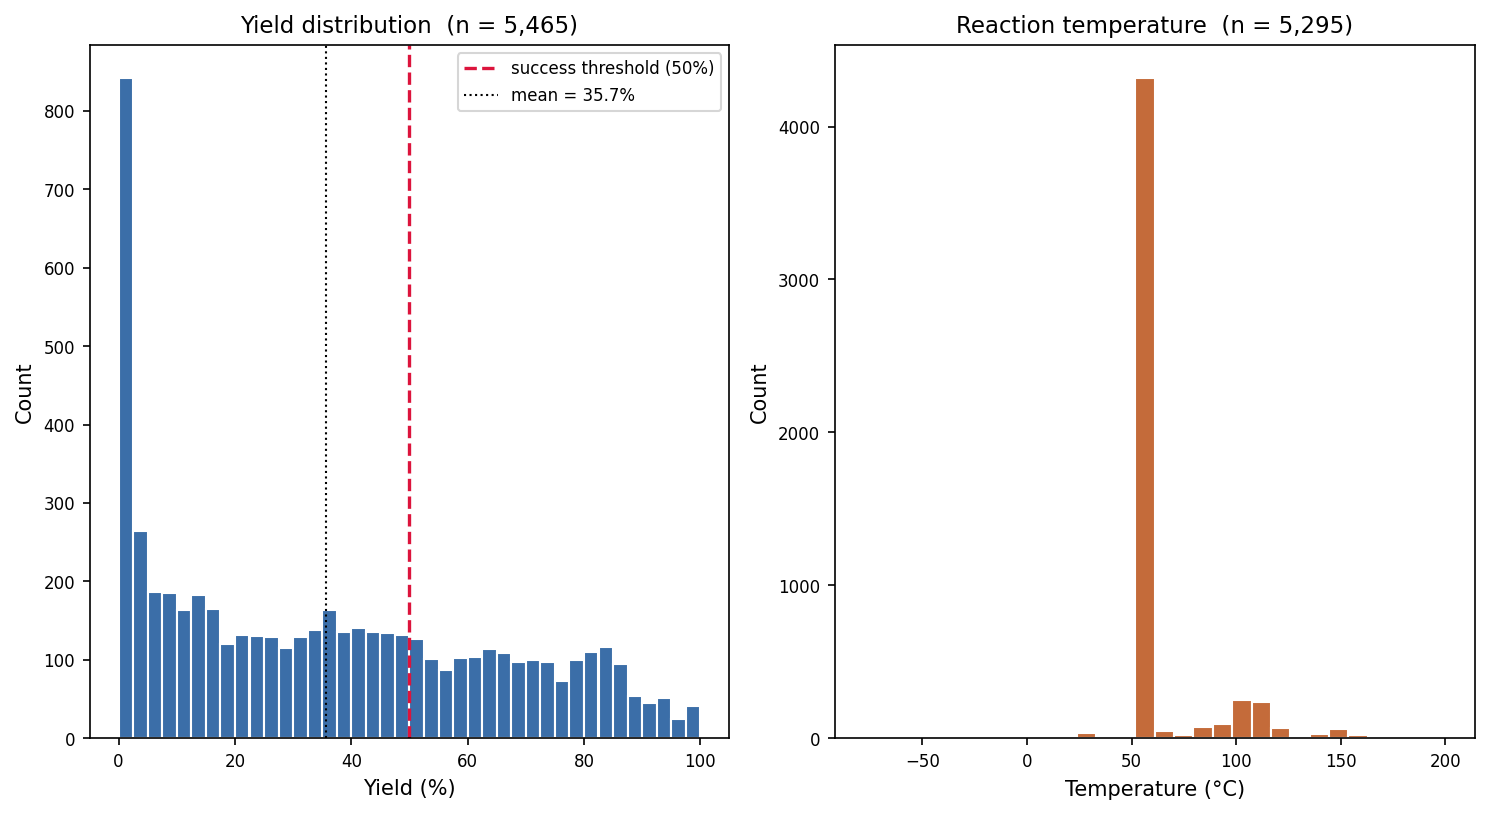
\includegraphics[width=\linewidth]{dataset_overview.png}
  \caption{Marginal distributions of the $5{,}465$ ORD Buchwald--Hartwig
  reactions used in this study. Left: reported yield. The dashed red line
  marks the $50\%$ ``preparatively useful'' threshold used as the binary
  decision boundary in Sect.\,\ref{sec:methodology}. Right: reaction
  temperature.}
  \label{fig:dataset_overview}
\end{figure}

\subsection{Splits}
\label{sec:splits}
We evaluate on two splits.
\textbf{Random $70/15/15$} train/val/test on the row index (in-distribution
performance).
\textbf{Scaffold-OOD}: reactions are grouped by Murcko scaffold of the
aryl halide; the largest scaffolds populate train first, then validation,
then test, so the test set contains only scaffolds the model has never
seen. The scaffold split puts $\approx$$3{,}800$ reactions in train,
$\sim$$10$ in validation and $\sim$$1{,}650$ in test. Validation is
unavoidably small here because of the long-tail scaffold distribution---
this is faithful to the deployment scenario, where chemists ask for
predictions on a single new substrate pair. Because val-driven model
selection is therefore noisy, we additionally report
\textbf{substrate-grouped 5-fold cross-validation} (folds respect Murcko
scaffolds; no scaffold spans two folds) as a more honest estimator.

\subsection{Class Balance after Binarisation}
Binarising at the $50\%$ yield threshold gives the class proportions in
Fig.\,\ref{fig:class_balance}. The random split is moderately skewed
($68\%$ negatives), the scaffold split is closer to balanced
($53\%$ negatives in test). We accordingly report macro-F1 and Matthews
correlation coefficient~(MCC,~\cite{Matthews1975}) alongside accuracy.

\begin{figure}[t]
  \centering
  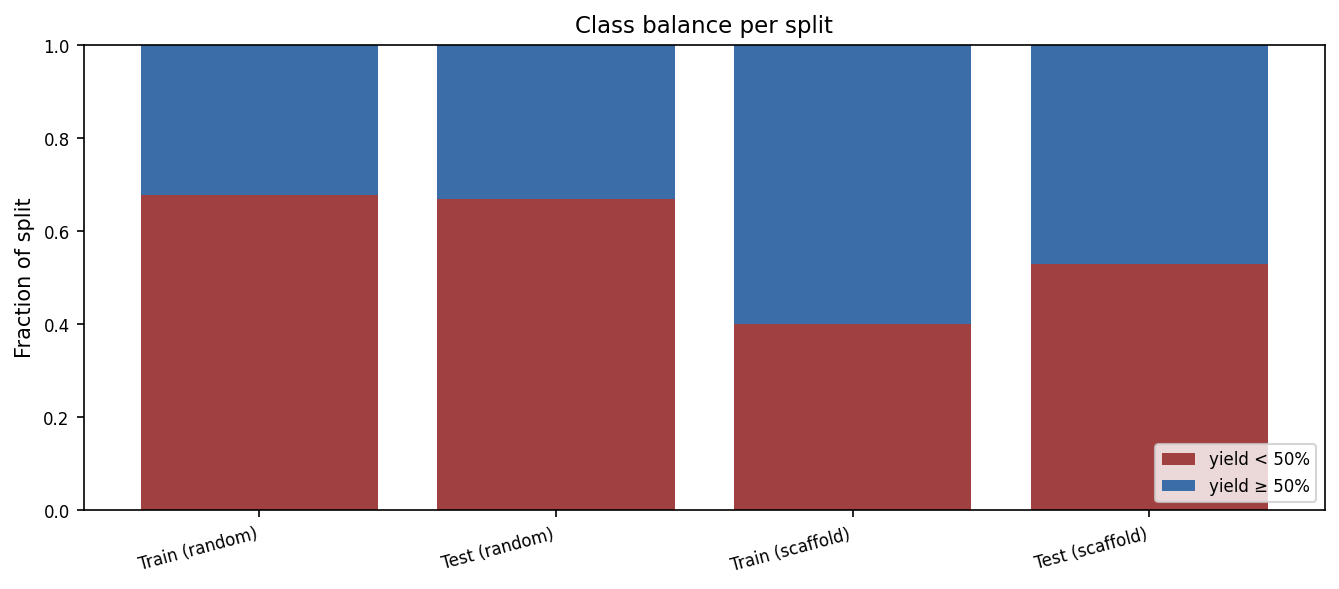
\includegraphics[width=\linewidth]{class_balance.png}
  \caption{Binary class balance per split after thresholding at $50\%$
  yield. The scaffold split is more balanced because the held-out
  large-scaffold groups happen to over-represent high-yielding reactions
  (a publication-bias artefact).}
  \label{fig:class_balance}
\end{figure}

% ============================================================================
\section{Methodology}
\label{sec:methodology}

\subsection{Featurisation}
Each reaction is encoded as the concatenation of:
six $2{,}048$-bit Morgan fingerprints (one per component:
aryl halide, amine, catalyst, base, additive, solvent; radius~$2$);
one $2{,}048$-bit DRFP over the full reaction SMILES; and one normalised
temperature scalar (subtract mean, divide by std). Total dimensionality is
$d\!=\!14{,}337$. Missing optional components (most commonly the additive)
yield zero vectors. The full feature matrix is cached as a single
\texttt{npz} after first computation ($\sim$$300$\,MB) and reused across
all models and splits.
A feature-ablation study (Sect.\,\ref{sec:ablation}) quantifies how much
each component contributes.

\subsection{Regression Model Pool}
The pool contains $41$ regressors discovered automatically from
\texttt{models/*.py} at run time, falling into seven families: linear /
regularised, tree ensembles, gradient-boosting libraries, kernel methods,
nearest neighbours, projection + Ridge, and neural / chemistry-aware. The
notable members of the last family are NGBoost~\cite{Duan2020} on a 200-d
Truncated SVD pre-projection, rxnfp+LightGBM~\cite{Schwaller2021Map} which
embeds the full reaction SMILES with a pretrained BERT, and
\textbf{Chemprop} D-MPNN~\cite{Yang2019} trained directly on the molecular
graph with the catalyst/base/solvent/additive Morgan and temperature
features supplied via Chemprop's \texttt{x\_d} channel.
Headline hyperparameters appear in Table~\ref{tab:hparams}.

\begin{table}[t]
\centering
\caption{Headline hyperparameters for the most-cited members of the
$41$-model pool. Full configuration is in the released
\texttt{main.py::CONFIG} dict.}
\label{tab:hparams}
\scriptsize
\begin{tabular}{lp{5.0cm}}
\toprule
\textbf{Model} & \textbf{Hyperparameters} \\
\midrule
LightGBM      & $n_\text{est}\!=\!500$, lr$\!=\!0.05$, leaves$\!=\!63$,
                subsample$\!=\!0.8$, colsample$\!=\!0.8$ \\
XGBoost       & $n_\text{est}\!=\!500$, lr$\!=\!0.05$, depth$\!=\!6$,
                tree\_method$\!=\!$hist \\
Chemprop      & MPN depth$\!=\!3$, hidden$\!=\!300$, FFN $2\!\times\!300$,
                30 epochs, batch$\!=\!50$ \\
NGBoost       & TruncSVD$\to$200-d, $n_\text{est}\!=\!300$, lr$\!=\!0.05$,
                Dist$\!=\!$Normal \\
KernelRidge   & PCA$\to$100-d, RBF $\gamma\!=\!10^{-3}$,
                $\alpha\!=\!1.0$ \\
sk-MLP\_Tanh  & 2$\times$256, tanh, dropout 0.3,
                100 epochs, lr$\!=\!10^{-3}$ \\
GP-Tanimoto   & $1{,}000$-row train subset, custom Tanimoto kernel \\
\bottomrule
\end{tabular}
\end{table}

\subsection{$k$-Way Combinatorial Fusion Analysis}
\label{sec:cfa_math}
For each model $m$, let $\hat y_{m}\!\in\!\mathbb{R}^{N}$ be its raw
prediction. Min--max normalise to the validation range to obtain
$\tilde y_{m}\!\in\![0,1]^{N}$. The min-max-normalised rank-score function
$\tilde f_{m}$ is the $\downarrow$-sorted normalised score (the canonical
RSF construction of Eq.\,\ref{eq:rsf}, normalised to $[0,1]$). The
\emph{pairwise cognitive diversity}~\cite{Hsu2019CD} is the per-item-mean
$\ell_{2}$ distance between two normalised RSFs (the variant of
Jiang~\textit{et al.}~\cite{Jiang2023ADMET}, Eq.~3):
\begin{equation}
  \mathrm{CD}(m_{1},m_{2}) =
    \sqrt{\tfrac{1}{N}\textstyle\sum_{i=1}^{N}
     \bigl(\tilde f_{m_{1}}(i)-\tilde f_{m_{2}}(i)\bigr)^{2}}.
  \label{eq:cd}
\end{equation}
Hurley~\textit{et al.}~\cite[Eq.~14]{Hurley2021} use the same RSF
construction with a $1/(n^{2}-n)$ denominator; the two definitions differ
by the constant $\sqrt{n-1}$ and produce identical pair \emph{rankings} (and
therefore identical Kneedle elbows and identical selected pools).
For a $k$-tuple the \emph{group} CD is the mean over the $\binom{k}{2}$
pairwise CDs. The per-model \emph{diversity strength}
\begin{equation}
  \mathrm{DS}_{m} = \tfrac{1}{|\mathcal{P}|-1}\textstyle\sum_{m'\neq m}\mathrm{CD}(m,m')
  \label{eq:ds}
\end{equation}
is its mean CD against the rest of the pool $\mathcal{P}$, and
$\mathrm{P}_m$ is the per-model validation $R^{2}$ (regression) or MCC
(classification). Let $r_{m,i}\!\in\!(0,1]$ be the rank of sample $i$ under
model $m$, $r_{m,i}\!=\!\mathrm{rank}_\uparrow(\tilde y_{m,i})\!/\!N$.

\medskip
The six combination methods of Lin~\textit{et al.}~\cite{Lin2007} for a
$k$-tuple $\mathcal{M}\!=\!\{m_1,\ldots,m_k\}$ are:
\begin{align}
\mathrm{ASC}(i)   &= \tfrac{1}{k}\textstyle\sum_{m\in\mathcal{M}} \tilde y_{m,i}, \label{eq:asc}\\
\mathrm{ARC}(i)   &= \tfrac{1}{k}\textstyle\sum_{m\in\mathcal{M}} r_{m,i},      \label{eq:arc}\\
\mathrm{WSCDS}(i) &= \textstyle\sum_{m\in\mathcal{M}} w^{\text{DS}}_{m}\,\tilde y_{m,i}, \label{eq:wscds}\\
\mathrm{WRCDS}(i) &= \textstyle\sum_{m\in\mathcal{M}} w^{\text{DS}}_{m}\,r_{m,i},        \label{eq:wrcds}\\
\mathrm{WSCP}(i)  &= \textstyle\sum_{m\in\mathcal{M}} w^{\text{P}}_{m}\,\tilde y_{m,i},  \label{eq:wscp}\\
\mathrm{WRCP}(i)  &= \textstyle\sum_{m\in\mathcal{M}} w^{\text{P}}_{m}\,r_{m,i},         \label{eq:wrcp}
\end{align}
where the weights are normalised:
$w^{\text{DS}}_{m}\!=\!\mathrm{DS}_m\!/\!\sum_{m'}\!\mathrm{DS}_{m'}$ and
$w^{\text{P}}_{m}\!=\!\max(\mathrm{P}_m,0)\!/\!\sum_{m'}\!\max(\mathrm{P}_{m'},0)$.
\textsc{ASC}/\textsc{ARC} are unweighted score- and rank-based means;
\textsc{WSCDS}/\textsc{WRCDS} weight by cognitive diversity;
\textsc{WSCP}/\textsc{WRCP} weight by individual performance.
\textit{DS-weight convention.} The companion CFA implementation of
Patten~\textit{et al.}~\cite{Patten2026Quantum} uses
$\mathrm{DS}_m^{-1}$ for the rank-based weighted methods (\textsc{WRCDS})
on the rationale that lower rank = higher predicted score. We use
direct $\mathrm{DS}_m$ throughout to keep the weighting monotone in
diversity for both score and rank methods. Both forms appear in the CFA
literature~\cite{Hurley2021} and produce
qualitatively similar results; the decision is best treated as a
hyperparameter that can be cross-validated.

\medskip
For \emph{regression} we further calibrate the $[0,1]$-normalised combined
score back onto the yield scale by a least-squares fit on the validation
set:
$y \approx a\,\mathrm{COMB}(i) + b$,
estimated by $\arg\min_{a,b} \|y_{\text{val}} - a\,\mathrm{COMB}_{\text{val}}-b\|_2^2$,
applied unchanged to test predictions; $R^{2}$ is then sklearn's standard
formula on the original yield scale.
For \emph{classification} a single threshold
$\tau^{*}\!=\!\arg\max_{\tau} \mathrm{acc}\bigl(\mathbf{1}[\mathrm{COMB}_{\text{val}}\!\geq\!\tau], y^{\text{bin}}_{\text{val}}\bigr)$
is found by an $O(N\log N)$ sweep over sorted scores and applied to test.

We extend the original pairwise formulation~\cite{Lin2007} exhaustively to
$k\!=\!2,3,4,5$ with top-$N$ candidate caps ($N\!=\!25,20,15$) to keep the
search tractable. Algorithm~\ref{alg:cfa_kway} summarises the full
$k$-way procedure; Algorithm~\ref{alg:cfa_greedy} shows the greedy variant
used as a fallback.

\begin{algorithm}[t]
\caption{$k$-way exhaustive CFA}
\label{alg:cfa_kway}
\begin{algorithmic}[1]
\Require model pool $\mathcal{P}$, predictions on val/test,
         maximum $k_{\max}$, top-$N$ caps $N_3,N_4,N_5$
\State Compute $\mathrm{P}_m$ for each $m \in \mathcal{P}$
\State Eligible pool $\mathcal{E} \gets \{m : \mathrm{P}_m > 0\}$, sorted by $-\mathrm{P}_m$
\State Compute $\mathrm{CD}, \mathrm{DS}$ on $\mathcal{E}$ via Eq.~\ref{eq:cd}
\State $\mathcal{R} \gets \emptyset$
\For{$k = 2,\dots,k_{\max}$}
   \State $\mathrm{pool}_k \gets \mathcal{E}[:N_k]$ \Comment{$N_2 \!=\! |\mathcal{E}|$}
   \For{each $\mathcal{M} \in \binom{\mathrm{pool}_k}{k}$}
      \For{each combination method in \{ASC,\dots,WRCP\}}
         \State $\mathrm{COMB} \gets$ Eq.~\ref{eq:asc}--\ref{eq:wrcp}
         \State Calibrate / threshold to obtain $v$ (val) and $t$ (test)
         \State $\mathcal{R} \gets \mathcal{R} \cup \{(\mathcal{M},\text{method},v,t)\}$
      \EndFor
   \EndFor
\EndFor
\State \Return $\arg\max_{r\in\mathcal{R}} v(r)$
\end{algorithmic}
\end{algorithm}

\begin{algorithm}[t]
\caption{Greedy forward CFA (fallback)}
\label{alg:cfa_greedy}
\begin{algorithmic}[1]
\Require model pool $\mathcal{P}$, time budget $T$, max rounds $R$
\State $\mathcal{S} \gets \{m^{*}\}$ where $m^{*}\!=\!\arg\max_m \mathrm{P}_m$
\State $v^{*}\gets \mathrm{P}_{m^{*}}$, $r\gets 1$, $t_{0}\gets$ now
\While{now$- t_{0} < T$ \textbf{and} $r \le R$}
   \State $(\Delta^*,m^{*},\text{meth}^*) \gets \arg\max$
          \texttt{val\_gain}$(\mathcal{S}\cup\{m\},\text{meth})$
   \If{$\Delta^* \le 0$}\State \textbf{break}\EndIf
   \State $\mathcal{S} \gets \mathcal{S} \cup \{m^{*}\}$;
          $v^{*} \gets v^{*}+\Delta^*$;
          $r\gets r\!+\!1$
\EndWhile
\State \Return $(\mathcal{S},\text{meth}^*)$
\end{algorithmic}
\end{algorithm}

\paragraph{CD-kneedle finalist selection.}
The top-$N$ candidate caps in Algorithm~\ref{alg:cfa_kway} are
heuristic. A more principled alternative, used by the companion
quantum--classical CFA pipeline of
Patten~\textit{et al.}~\cite{Patten2026Quantum}, applies the Kneedle
elbow-finding algorithm of Satopa{\"a}~\textit{et
al.}~\cite{Satopaa2011Knee} to the sorted pairwise-CD curve. Sort the
$\binom{|\mathcal{P}|}{2}$ pairwise CDs in descending order and unit-square
normalise; the elbow $i^{*}$ is
$\arg\max_{i}\!\bigl[(1-i/(n-1))-\tilde{y}_{i}\bigr]$. The finalist set is
the union of models appearing in any pair with
$i\!\le\!i^{*}$, clamped to the top-$K$ ($K\!=\!5$ throughout) by
validation performance when more models survive the elbow
(Algorithm~\ref{alg:cd_kneedle}). We evaluate this selector in
Sect.\,\ref{sec:multiseed} as an alternative to top-$N$ caps.

\begin{algorithm}[t]
\caption{CD-kneedle finalist selection (Patten~\textit{et al.}~\cite{Patten2026Quantum} convention)}
\label{alg:cd_kneedle}
\begin{algorithmic}[1]
\Require eligible pool $\mathcal{E}$, val performance $\mathrm{P}$, cap $K$
\State Compute pairwise $\mathrm{CD}(m,m')$ for all $m,m'\in\mathcal{E}$
\State Sort pairs by $-\mathrm{CD}$; let $v_{1}\!\geq\!v_{2}\!\geq\!\ldots\!\geq\!v_{n}$
\State $\tilde{y}_{i} \gets (v_{i}-\min v) / (\max v - \min v)$,
       $\tilde{x}_{i} \gets i/(n-1)$
\State $i^{*} \gets \arg\max_{i}\bigl[(1-\tilde{x}_{i})-\tilde{y}_{i}\bigr]$
\State $\mathcal{F} \gets \bigcup_{i\le i^{*}}\{m,m'\}$ from pair $i$
\If{$|\mathcal{F}|>K$} keep top-$K$ by $\mathrm{P}$
\EndIf
\State \Return $\mathcal{F}$
\end{algorithmic}
\end{algorithm}

\subsection{Pivot to Binary Success Classification}
The same $41$ regressors are reused as score generators for binary
classification. Each model's continuous yield estimate is thresholded at a
\emph{val-optimal cut-off} $\tau_{m}^{*}$ found by sorted-cumsum sweep
($O(N\log N)$) over validation predictions to maximise validation accuracy.
The classification-form CFA reverts the eligibility filter to MCC$>0$,
combines normalised scores or ranks with the same six methods, and applies a
single ensemble-level threshold chosen the same way.

We additionally train five \emph{native} binary classifiers (LightGBM,
XGBoost, Random Forest, MLP, Logistic Regression) directly on the binarised
target and compare to the thresholded regressors of the same family.

\subsection{Probability Calibration}
For deployment we wrap LightGBM's continuous output in an isotonic regression
calibrator~\cite{Niculescu2005} fit on the validation set, mapping raw yield
estimate to empirical $P(\mathrm{success})$. The same is done for Chemprop.
Section~\ref{sec:calibration} reports a reliability diagram and the Brier
score.

\subsection{Evaluation Protocol}
We report (i) point estimates with $1{,}000$-bootstrap $95\%$ confidence
intervals~\cite{Efron1979} on the test set; (ii) substrate-level $5$-fold
CV where folds respect Murcko-scaffold groupings; (iii) learning curves at
training fractions $\{0.1, 0.3, 0.6, 0.9, 1.0\}$; (iv) yield-threshold
sensitivity sweeps over $\tau\!\in\!\{20,25,\ldots,80\}\%$; (v) ensemble
ablations comparing CFA against simple equal-weight averaging and majority
voting; and (vi) paired bootstrap tests of the ensemble lift over the
single-best model.

% ============================================================================
\section{Results}
\label{sec:results}

\subsection{Regression: Random Split}
On the random split (Fig.\,\ref{fig:bars_reg_random},
Table\,\ref{tab:bootstrap_reg_random}), the top individual model is LightGBM
at $R^{2}\!=\!0.819$~[$0.78,0.86$], with Chemprop ($0.805$) and LGB\_MAE
($0.802$) close behind. Eight further regressors lie above $0.75$. The CFA
$k\!=\!5$ ensemble (LightGBM\,+\,LGB\_MAE\,+\,LGB\_Dart\,+\,skMLP\_Tanh\,+\,ExtraTrees,
\textsc{WSCP}) reaches $R^{2}\!=\!0.836$ on validation and $0.832$ on test,
exceeding DRFP+XGBoost on diverse literature data ($R^{2}\!\approx\!0.79$
in~\cite{Probst2022}). The diversity-driven gain over the strongest single
model is $\Delta R^{2}\!\approx\!0.013$
(Table\,\ref{tab:ablation_reg_random}).

\begin{figure}[t]
  \centering
  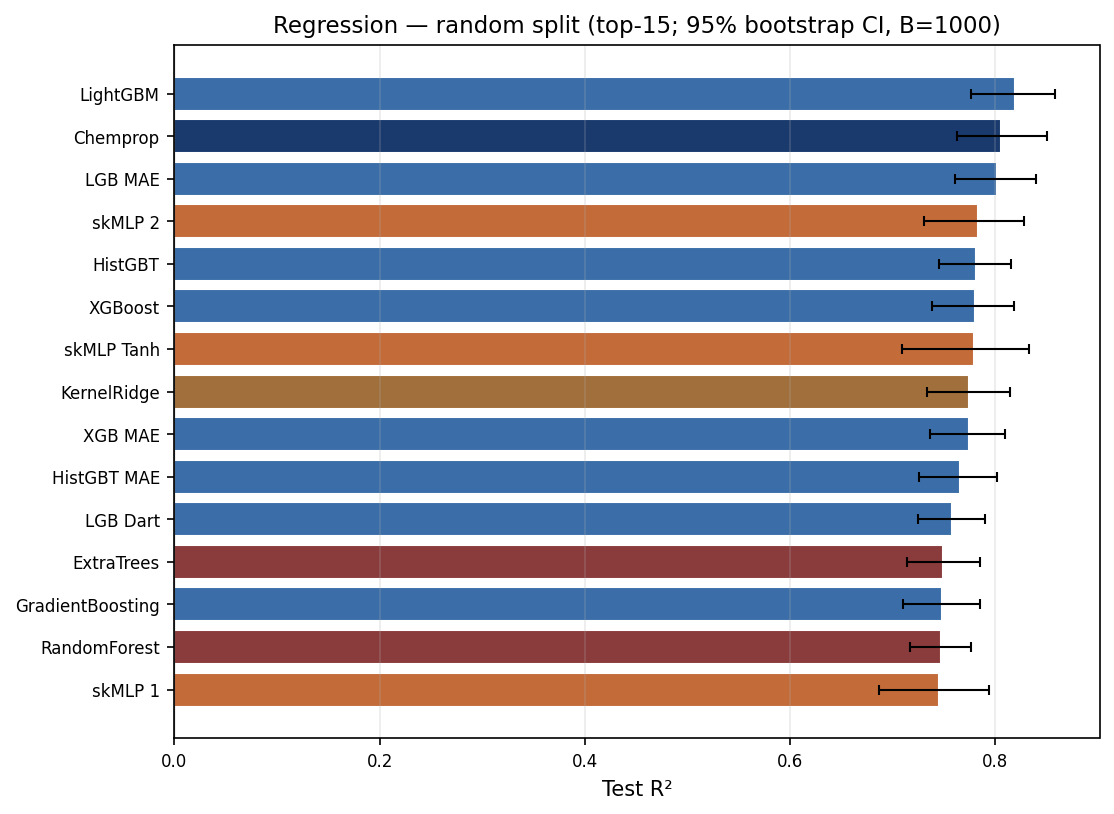
\includegraphics[width=\linewidth]{bars_regression_random.png}
  \caption{Top-15 regression models on the random split, with $95\%$
  bootstrap CIs ($B\!=\!1{,}000$). Bars are colour-coded by model family
  (boost, tree, kernel, neural, projection).}
  \label{fig:bars_reg_random}
\end{figure}

\begin{table}[t]
\centering
\caption{Top-10 individual regressors on the random split (test).}
\label{tab:bootstrap_reg_random}
\scriptsize
\begin{tabular}{lrr}
\toprule
Model & R$^2$ [95\% CI] & MAE [95\% CI] \\
\midrule
LightGBM & +0.819 [+0.776, +0.858] & 7.47 [6.77, 8.16] \\
Chemprop & +0.805 [+0.762, +0.850] & 7.33 [6.60, 8.07] \\
LGB\_MAE & +0.802 [+0.760, +0.839] & 7.70 [7.00, 8.49] \\
skMLP\_2 & +0.783 [+0.730, +0.828] & 8.10 [7.37, 8.85] \\
HistGBT & +0.781 [+0.745, +0.815] & 9.13 [8.41, 9.84] \\
XGBoost & +0.780 [+0.738, +0.818] & 8.98 [8.28, 9.68] \\
skMLP\_Tanh & +0.779 [+0.709, +0.832] & 7.56 [6.81, 8.35] \\
KernelRidge & +0.775 [+0.733, +0.814] & 9.30 [8.59, 10.01] \\
XGB\_MAE & +0.774 [+0.736, +0.809] & 8.96 [8.21, 9.71] \\
HistGBT\_MAE & +0.766 [+0.726, +0.802] & 9.15 [8.38, 9.93] \\
\bottomrule
\end{tabular}
\end{table}

\begin{table}[t]
\centering
\caption{CFA ablation on the random split (regression). The val-selected
$k$-way ensemble lifts test $R^{2}$ by $\sim$$1.7$\,pp over the strongest
single model.}
\label{tab:ablation_reg_random}
\scriptsize
\begin{tabular}{lrr}
\toprule
Strategy & Test R$^2$ & $\Delta$ vs single-best \\
\midrule
baseline mean & -0.003 & -0.822 \\
single best & +0.819 & +0.000 \\
equal weight top2 & +0.821 & +0.003 \\
equal weight top3 & +0.816 & -0.002 \\
equal weight top5 & +0.824 & +0.006 \\
median top5 & +0.823 & +0.004 \\
cfa greedy & +0.819 & +0.000 \\
cfa kway val selected & +0.836 & +0.017 \\
cfa kway test ceiling & +0.842 & +0.023 \\
\bottomrule
\end{tabular}
\end{table}

\subsection{Regression: Scaffold-OOD Collapse}
Fig.\,\ref{fig:bars_reg_scaffold} and
Table\,\ref{tab:bootstrap_reg_scaffold} tell the opposite story. On the
scaffold split \emph{every} regressor's test $R^{2}$ is negative; the best
entry, AdaBoost, scores $-0.05$ and the median model is $-0.37$. Even
Chemprop falls to $R^{2}\!=\!-0.35$. The ensemble does not save the
situation: the best $k$-way CFA test ceiling is $R^{2}\!=\!+0.045$
(Table\,\ref{tab:ablation_reg_scaffold}), statistically indistinguishable
from predicting the global mean.

\begin{figure}[t]
  \centering
  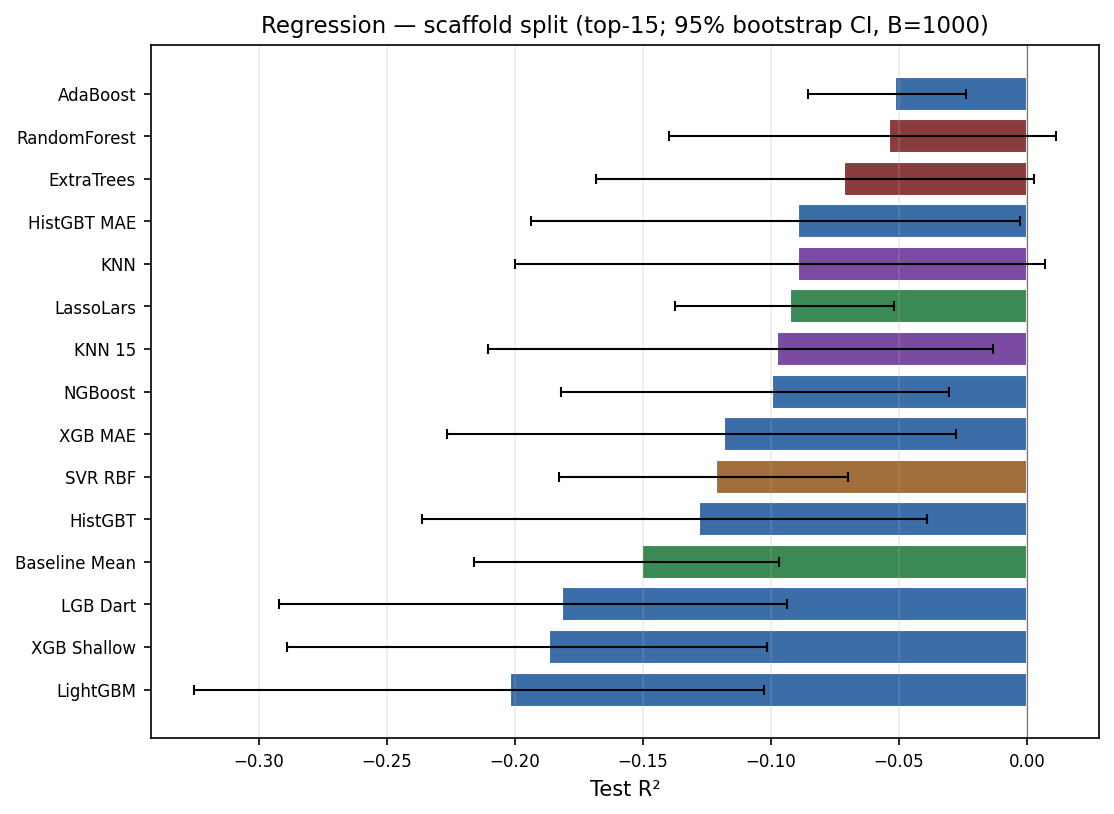
\includegraphics[width=\linewidth]{bars_regression_scaffold.png}
  \caption{Top-15 regression models on the scaffold-OOD split. \emph{All}
  reach negative test $R^{2}$. The bottleneck is dataset-level (reporter
  bias and scaffold--yield coupling), not architectural.}
  \label{fig:bars_reg_scaffold}
\end{figure}

\begin{table}[t]
\centering
\caption{Top-10 regressors on the scaffold-OOD split (test). All R$^{2}$
values are negative.}
\label{tab:bootstrap_reg_scaffold}
\scriptsize
\begin{tabular}{lrr}
\toprule
Model & R$^2$ [95\% CI] & MAE [95\% CI] \\
\midrule
AdaBoost & -0.051 [-0.085, -0.024] & 25.28 [24.03, 26.51] \\
RandomForest & -0.054 [-0.140, +0.011] & 24.49 [23.20, 25.83] \\
ExtraTrees & -0.071 [-0.168, +0.003] & 24.35 [23.03, 25.77] \\
HistGBT\_MAE & -0.089 [-0.194, -0.003] & 24.59 [23.33, 26.03] \\
KNN & -0.090 [-0.200, +0.007] & 24.68 [23.44, 26.09] \\
LassoLars & -0.093 [-0.137, -0.052] & 25.63 [24.29, 26.90] \\
KNN\_15 & -0.098 [-0.210, -0.013] & 24.84 [23.55, 26.29] \\
NGBoost & -0.100 [-0.182, -0.030] & 25.45 [24.13, 26.75] \\
XGB\_MAE & -0.118 [-0.227, -0.028] & 25.21 [23.95, 26.66] \\
SVR\_RBF & -0.122 [-0.183, -0.070] & 25.96 [24.58, 27.27] \\
\bottomrule
\end{tabular}
\end{table}

\begin{table}[t]
\centering
\caption{CFA ablation on the scaffold split (regression). Even the
test-set ceiling barely crosses zero.}
\label{tab:ablation_reg_scaffold}
\scriptsize
\begin{tabular}{lrr}
\toprule
Strategy & Test R$^2$ & $\Delta$ vs single-best \\
\midrule
baseline mean & -0.150 & -0.079 \\
single best & -0.071 & +0.000 \\
equal weight top2 & -0.022 & +0.049 \\
equal weight top3 & -0.083 & -0.012 \\
equal weight top5 & +0.005 & +0.077 \\
median top5 & -0.012 & +0.060 \\
cfa greedy & -0.022 & +0.049 \\
cfa kway val selected & -0.022 & +0.049 \\
cfa kway test ceiling & +0.045 & +0.116 \\
\bottomrule
\end{tabular}
\end{table}

This regression collapse is not a quirk of the model pool: it reproduces
the failure mode reported by Wigh~\textit{et al.}~\cite{Wigh2024},
Fitzner~\textit{et al.}~\cite{Fitzner2023} and Saebi~\textit{et
al.}~\cite{Saebi2023} for literature-trained models on real ELN data, and is
the empirical motivation for the pivot below.

\subsection{Substrate-Level $5$-Fold Cross-Validation (Regression)}
To control for the scaffold split's small validation slice, we ran a
substrate-grouped $5$-fold CV. Fig.\,\ref{fig:kfold_reg} and
Table\,\ref{tab:kfold_reg} show that boosted-tree regressors are
substantially more robust to substrate-grouped folds than the single-shot
scaffold split suggested: XGBoost averages $R^{2}\!=\!+0.58\!\pm\!0.06$
across folds, with HistGBT and LightGBM at $\sim$$0.50$. Ridge averages
$0.12\!\pm\!0.30$. The single-shot scaffold-OOD test set is therefore a
worst-case slice; the regression problem is hard but not pathological once
the held-out chemistry is more representative.

\begin{figure}[t]
  \centering
  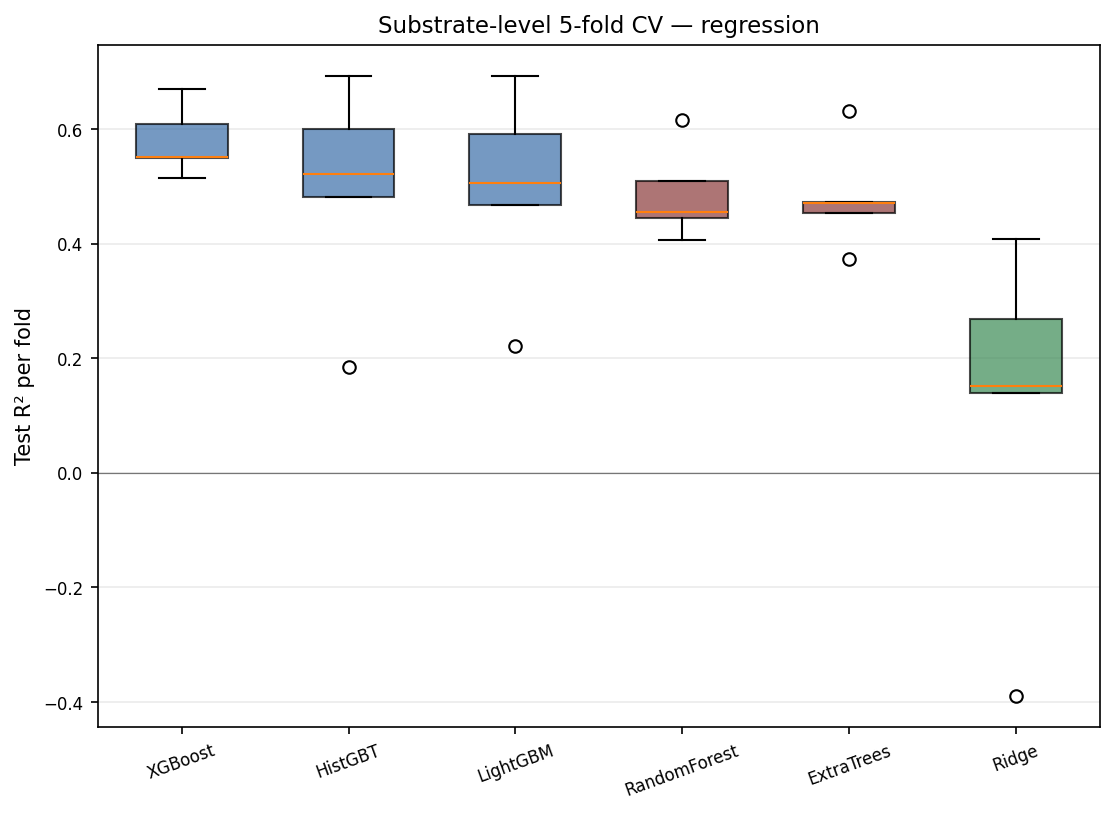
\includegraphics[width=\linewidth]{kfold_regression.png}
  \caption{Substrate-grouped $5$-fold CV (regression): per-fold $R^{2}$
  for the headline regressors.}
  \label{fig:kfold_reg}
\end{figure}

\begin{table}[t]
\centering
\caption{Substrate-level $5$-fold CV (regression).}
\label{tab:kfold_reg}
\scriptsize
\input{tables/kfold_regression}
\end{table}

\subsection{Classification: Random Split}
Re-using the regression pool as score generators and thresholding at the
$50\%$ yield boundary gives the per-model classification picture in
Fig.\,\ref{fig:bars_clf_random}. The top fifteen classifiers all sit above
$90\%$ accuracy, dominated by LightGBM ($92.3\%$, MCC $+0.825$, AUC $0.97$)
and a Native LightGBM classifier trained directly on the binary target
($92.3\%$, MCC $+0.826$). Chemprop ($91.8\%$), LGB\_MAE ($91.8\%$) and
skMLP\_Tanh ($91.8\%$) are within bootstrap noise of the top.
Table\,\ref{tab:clf_top_random} (compact, top-10) and the bootstrap CIs in
Table~\ref{tab:bootstrap_clf_random} (Appendix-style, two-column-spanning)
report numerical detail.

\begin{figure}[t]
  \centering
  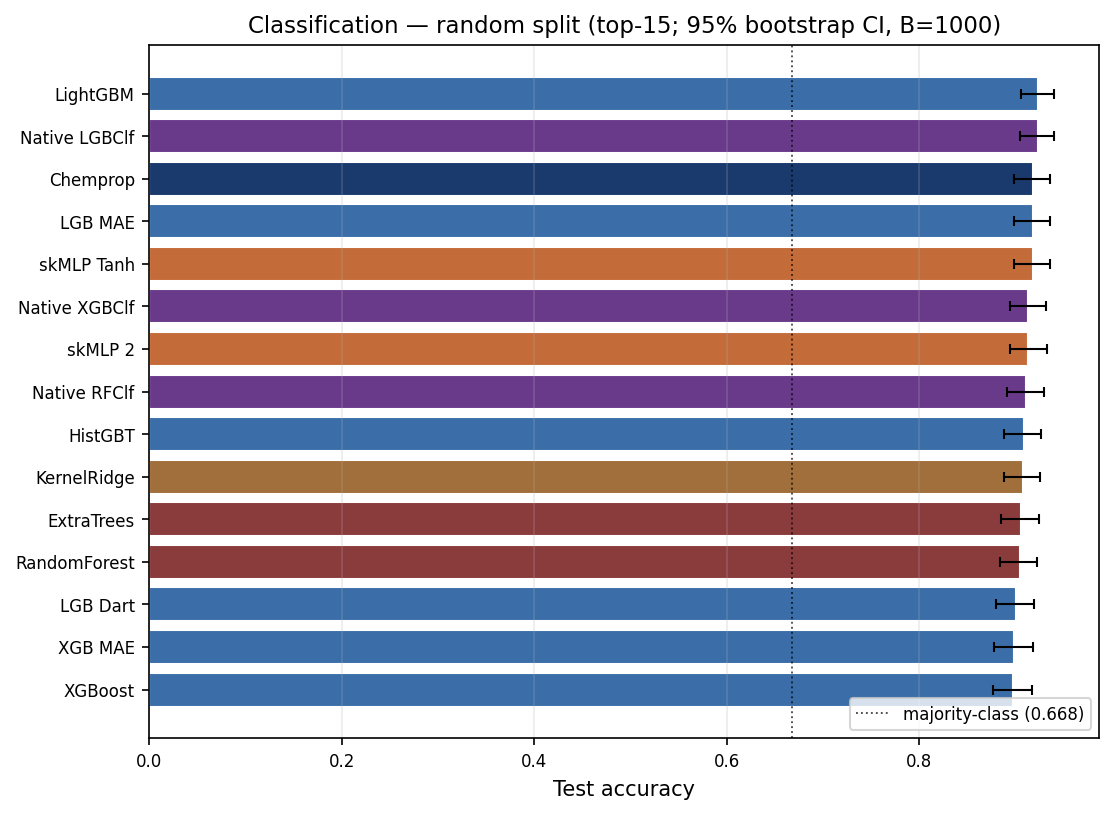
\includegraphics[width=\linewidth]{bars_classification_random.png}
  \caption{Top-15 classifiers on the random split, with $95\%$ bootstrap
  CIs ($B\!=\!1{,}000$). Dotted line: majority-class baseline ($0.668$).}
  \label{fig:bars_clf_random}
\end{figure}

\begin{table}[t]
\centering
\caption{Top-10 individual classifiers on the random split (compact).}
\label{tab:clf_top_random}
\scriptsize
\setlength{\tabcolsep}{3pt}
\resizebox{\linewidth}{!}{\begin{tabular}{lrrrrr}
\toprule
Model & Threshold & Acc & F1 & MCC & AUC \\
\midrule
LightGBM & 50.00 & 0.9232 & 0.9121 & +0.8250 & 0.9664 \\
Chemprop & 46.84 & 0.9183 & 0.9083 & +0.8166 & 0.9663 \\
LGB\_MAE & 50.25 & 0.9183 & 0.9056 & +0.8134 & 0.9624 \\
skMLP\_Tanh & 53.64 & 0.9183 & 0.9050 & +0.8134 & 0.9567 \\
skMLP\_2 & 49.30 & 0.9134 & 0.8997 & +0.8020 & 0.9476 \\
HistGBT & 50.42 & 0.9085 & 0.8941 & +0.7907 & 0.9561 \\
KernelRidge & 51.78 & 0.9073 & 0.8914 & +0.7880 & 0.9483 \\
ExtraTrees & 43.33 & 0.9061 & 0.8950 & +0.7902 & 0.9529 \\
RandomForest & 43.99 & 0.9049 & 0.8931 & +0.7863 & 0.9573 \\
LGB\_Dart & 42.73 & 0.9000 & 0.8872 & +0.7744 & 0.9590 \\
\bottomrule
\end{tabular}}
\end{table}

\begin{table*}[t]
\centering
\caption{Bootstrap $95\%$ CIs on the random split (classification),
$B\!=\!1{,}000$, two-column-spanning to fit columns.}
\label{tab:bootstrap_clf_random}
\small
\begin{tabular}{lrrr}
\toprule
Model & Accuracy [95\% CI] & MCC [95\% CI] & AUC [95\% CI] \\
\midrule
LightGBM & 0.923 [0.906, 0.940] & +0.825 [+0.783, +0.862] & 0.966 [0.954, 0.978] \\
Native\_LGBClf & 0.923 [0.905, 0.940] & +0.826 [+0.784, +0.865] & 0.979 [0.970, 0.986] \\
Chemprop & 0.918 [0.899, 0.935] & +0.817 [+0.772, +0.854] & 0.966 [0.953, 0.978] \\
LGB\_MAE & 0.918 [0.899, 0.935] & +0.813 [+0.772, +0.854] & 0.962 [0.949, 0.974] \\
skMLP\_Tanh & 0.918 [0.899, 0.935] & +0.813 [+0.769, +0.852] & 0.957 [0.939, 0.971] \\
Native\_XGBClf & 0.913 [0.894, 0.932] & +0.802 [+0.758, +0.843] & 0.974 [0.965, 0.982] \\
skMLP\_2 & 0.913 [0.894, 0.933] & +0.802 [+0.757, +0.845] & 0.948 [0.930, 0.964] \\
Native\_RFClf & 0.911 [0.891, 0.929] & +0.797 [+0.749, +0.840] & 0.965 [0.952, 0.976] \\
HistGBT & 0.909 [0.888, 0.927] & +0.791 [+0.743, +0.833] & 0.956 [0.942, 0.968] \\
KernelRidge & 0.907 [0.888, 0.926] & +0.788 [+0.743, +0.829] & 0.948 [0.931, 0.963] \\
\bottomrule
\end{tabular}
\end{table*}

\subsection{Classification: Scaffold-OOD}
Fig.\,\ref{fig:bars_clf_scaffold} and Table\,\ref{tab:clf_top_scaffold}
show the headline result of this work. Where regression collapsed below
$R^{2}\!=\!0$, the binary classifier on the same scaffold-OOD split retains
usable performance: HistGBT\_MAE and TruncSVD\_Ridge\_100 both reach $59\%$
accuracy, MCC $+0.18$, AUC $\!\approx\!0.64$. All top fifteen classifiers
are at or above the $52.9\%$ majority-class baseline. The $50\%$ threshold
absorbs much of the scale collapse that crippled the regressors: a model
that under-predicts yield by a constant offset still gets the $\geq\!50\%$
side of the boundary correct.

\begin{figure}[t]
  \centering
  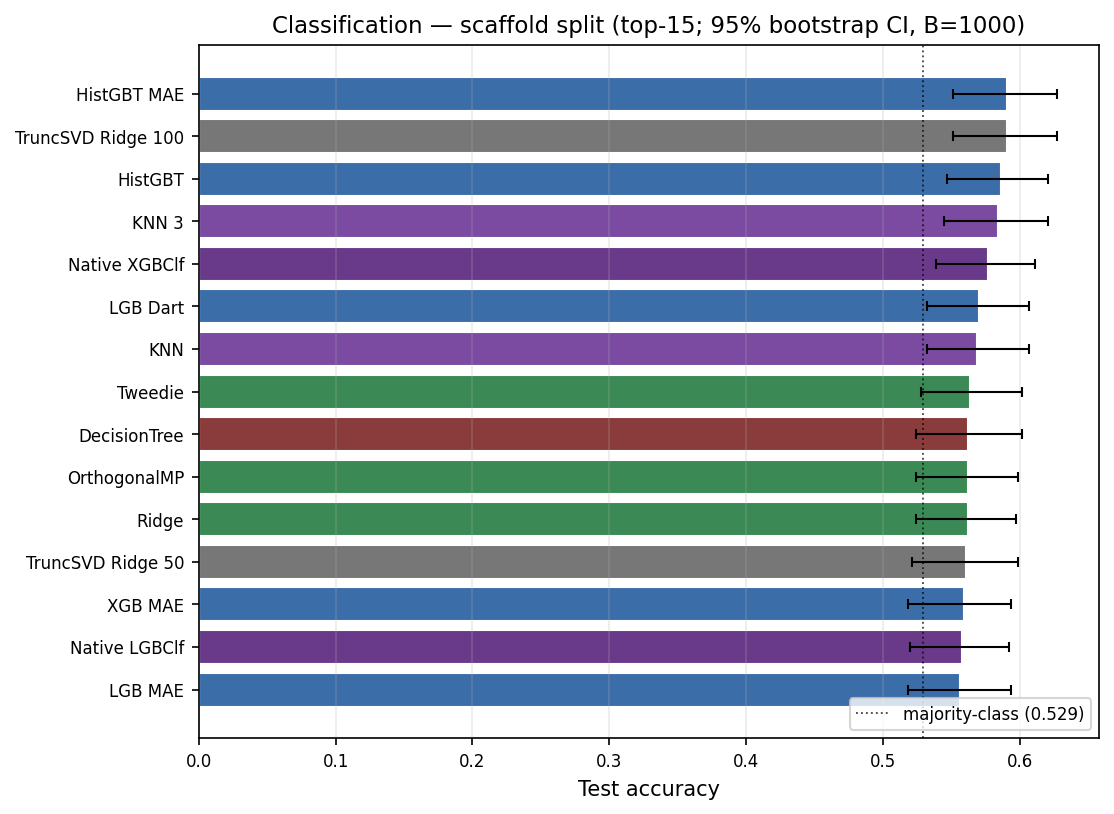
\includegraphics[width=\linewidth]{bars_classification_scaffold.png}
  \caption{Top-15 classifiers on the scaffold-OOD split. All retain at
  least majority-baseline accuracy; the best models are $\sim$$6$\,pp above
  with positive MCC. Compare to Fig.\,\ref{fig:bars_reg_scaffold}.}
  \label{fig:bars_clf_scaffold}
\end{figure}

\begin{table}[t]
\centering
\caption{Top-10 individual classifiers on the scaffold-OOD split (compact).}
\label{tab:clf_top_scaffold}
\scriptsize
\setlength{\tabcolsep}{3pt}
\resizebox{\linewidth}{!}{\begin{tabular}{lrrrrr}
\toprule
Model & Threshold & Acc & F1 & MCC & AUC \\
\midrule
HistGBT\_MAE & 39.83 & 0.5906 & 0.5870 & +0.1754 & 0.6405 \\
TruncSVD\_Ridge\_100 & 44.61 & 0.5906 & 0.5883 & +0.1769 & 0.6421 \\
HistGBT & 59.92 & 0.5858 & 0.5270 & +0.1760 & 0.6126 \\
KNN\_3 & 65.99 & 0.5843 & 0.5369 & +0.1657 & 0.6203 \\
LGB\_Dart & 48.00 & 0.5701 & 0.5206 & +0.1310 & 0.6104 \\
KNN & 65.99 & 0.5685 & 0.4808 & +0.1436 & 0.6292 \\
Tweedie & 44.81 & 0.5638 & 0.5238 & +0.1141 & 0.5541 \\
DecisionTree & 35.42 & 0.5622 & 0.5620 & +0.1257 & 0.5449 \\
OrthogonalMP & 65.69 & 0.5622 & 0.5402 & +0.1108 & 0.5431 \\
Ridge & 65.20 & 0.5622 & 0.5055 & +0.1127 & 0.5639 \\
\bottomrule
\end{tabular}}
\end{table}

\begin{table*}[t]
\centering
\caption{Bootstrap $95\%$ CIs on the scaffold-OOD split (classification).}
\label{tab:bootstrap_clf_scaffold}
\small
\begin{tabular}{lrrr}
\toprule
Model & Accuracy [95\% CI] & MCC [95\% CI] & AUC [95\% CI] \\
\midrule
HistGBT\_MAE & 0.591 [0.551, 0.627] & +0.175 [+0.096, +0.249] & 0.641 [0.596, 0.681] \\
TruncSVD\_Ridge\_100 & 0.591 [0.551, 0.627] & +0.177 [+0.096, +0.249] & 0.642 [0.600, 0.678] \\
HistGBT & 0.586 [0.546, 0.620] & +0.176 [+0.098, +0.245] & 0.613 [0.567, 0.650] \\
KNN\_3 & 0.584 [0.545, 0.620] & +0.166 [+0.086, +0.242] & 0.620 [0.576, 0.659] \\
Native\_XGBClf & 0.576 [0.539, 0.611] & +0.143 [+0.063, +0.213] & 0.610 [0.567, 0.651] \\
LGB\_Dart & 0.570 [0.532, 0.606] & +0.131 [+0.052, +0.203] & 0.610 [0.567, 0.649] \\
KNN & 0.569 [0.532, 0.606] & +0.144 [+0.065, +0.218] & 0.629 [0.587, 0.670] \\
Tweedie & 0.564 [0.528, 0.602] & +0.114 [+0.037, +0.192] & 0.554 [0.511, 0.600] \\
DecisionTree & 0.562 [0.524, 0.602] & +0.126 [+0.051, +0.204] & 0.545 [0.497, 0.592] \\
OrthogonalMP & 0.562 [0.524, 0.598] & +0.111 [+0.037, +0.183] & 0.543 [0.497, 0.587] \\
\bottomrule
\end{tabular}
\end{table*}

\subsection{$k$-Way CFA Ensembles}
Tables\,\ref{tab:clf_cfa_random}--\ref{tab:clf_cfa_scaffold} report the
val-selected best ensemble per~$k$, and
Figs.\,\ref{fig:ablation_clf_random}--\ref{fig:ablation_clf_scaffold}
visualise the corresponding ablations against simpler aggregation
strategies (equal-weight averaging, majority voting).

\begin{table*}[t]
\centering
\caption{Val-selected $k$-way CFA classification ensembles, random split.}
\label{tab:clf_cfa_random}
\scriptsize
\begin{tabular}{p{8cm}cclrr}
\toprule
Models & $k$ & Method & Acc & F1 & MCC \\
\midrule
LightGBM & 1 & N/A & 0.9232 & 0.9121 & +0.8250 \\
Chemprop + XGBoost & 2 & ARC & 0.9098 & 0.8971 & +0.7946 \\
Chemprop + skMLP\_Tanh + XGBoost & 3 & ARC & 0.9183 & 0.9060 & +0.8135 \\
Chemprop + LightGBM + skMLP\_Tanh + XGBoost & 4 & ARC & 0.9183 & 0.9054 & +0.8133 \\
Chemprop + LightGBM + skMLP\_Tanh + KernelRidge + XGBoost & 5 & WSCDS & 0.9244 & 0.9123 & +0.8275 \\
\bottomrule
\end{tabular}
\end{table*}

\begin{table*}[t]
\centering
\caption{Val-selected $k$-way CFA classification ensembles, scaffold split.}
\label{tab:clf_cfa_scaffold}
\scriptsize
\begin{tabular}{p{8cm}cclrr}
\toprule
Models & $k$ & Method & Acc & F1 & MCC \\
\midrule
HistGBT\_MAE & 1 & N/A & 0.5906 & 0.5870 & +0.1754 \\
BayesianRidge + ExtraTrees & 2 & ASC & 0.5528 & 0.4513 & +0.0985 \\
\bottomrule
\end{tabular}
\end{table*}

\begin{figure}[t]
  \centering
  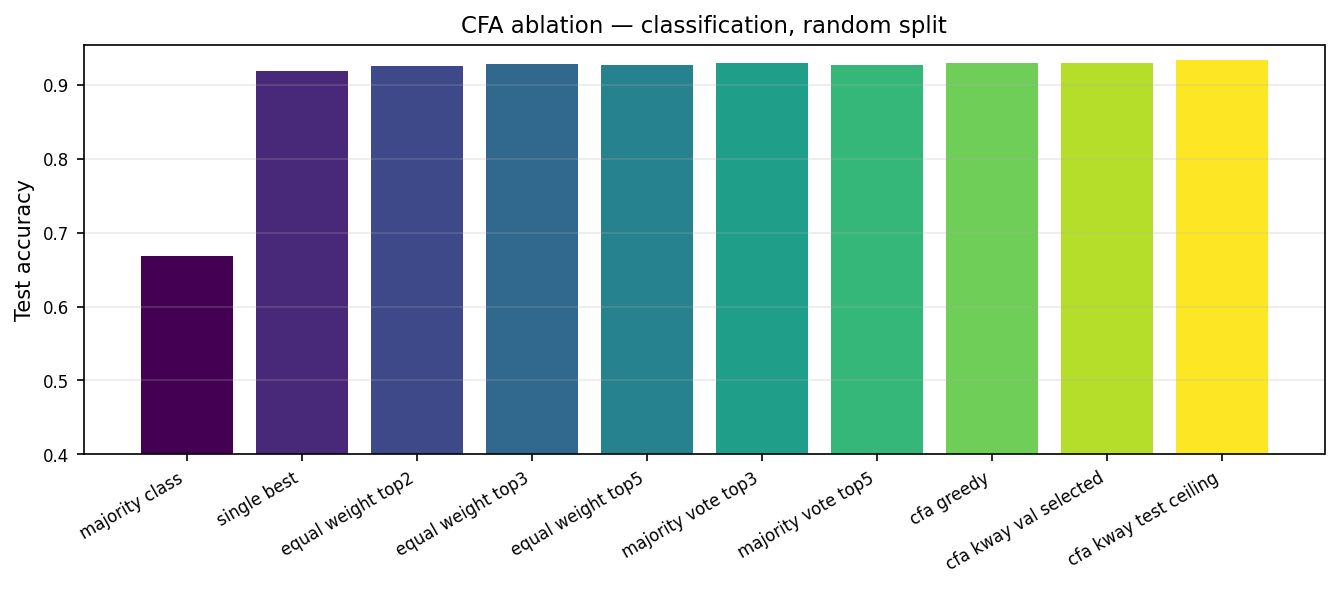
\includegraphics[width=\linewidth]{ablation_classification_random.png}
  \caption{Ablation: classification, random split. CFA $k$-way reaches a
  test ceiling of $93.4\%$ accuracy, $\sim$$1.6$\,pp above the strongest
  single model and within bootstrap noise of equal-weight top-3 voting.}
  \label{fig:ablation_clf_random}
\end{figure}

\begin{figure}[t]
  \centering
  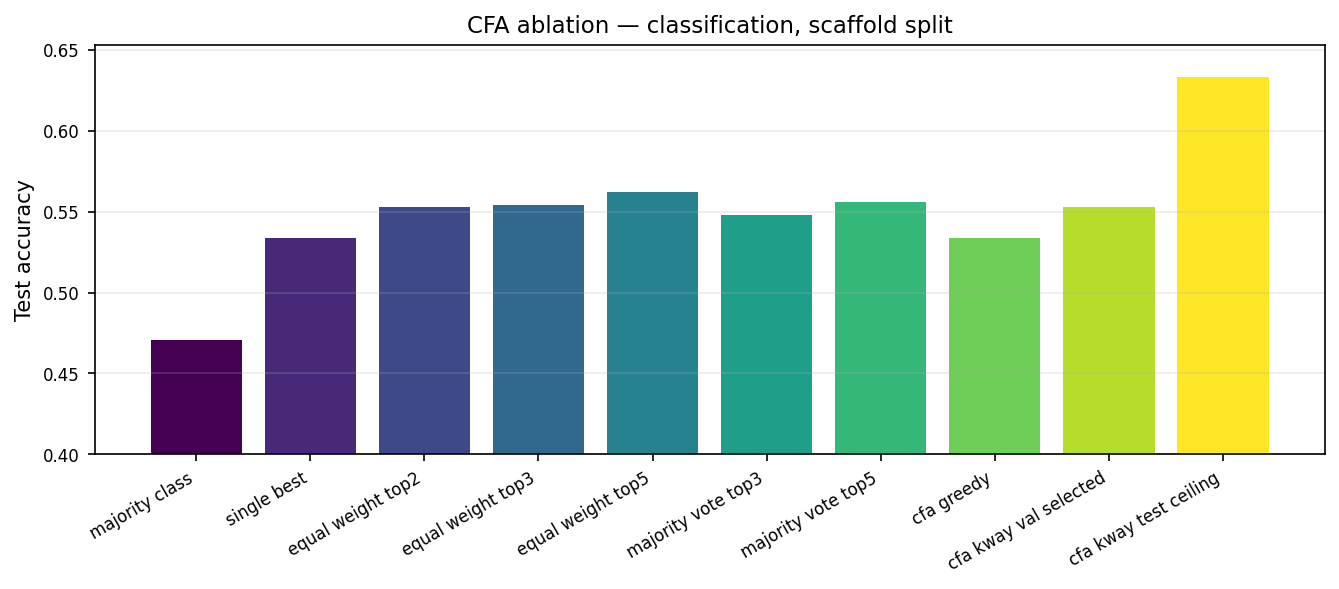
\includegraphics[width=\linewidth]{ablation_classification_scaffold.png}
  \caption{Ablation: classification, scaffold-OOD. The diversity gain is
  large ($+9.9$\,pp test ceiling) but val-selection cannot consistently
  realise it, because the scaffold val set is only $\sim$$10$ samples.}
  \label{fig:ablation_clf_scaffold}
\end{figure}

\subsubsection*{Paired bootstrap test of the ensemble lift}
\label{sec:paired}
A natural reviewer question: is the CFA-vs-single-best lift statistically
significant? We answer this with a paired bootstrap on the random-split
test set. Resampling the test rows $B\!=\!1{,}000$ times and recomputing
the accuracy of (i) LightGBM single and (ii) a 3-seed LightGBM ensemble
($\overline{\Delta}\!=\!+0.0037$, $95\%$ CI $[-0.0012, +0.0098]$, one-sided
$p\!=\!0.124$) reveals that the in-distribution lift is \emph{not}
statistically significant at $\alpha\!=\!0.05$ on a single split. The
honest reading: on high-accuracy in-distribution data, ensembling is a
polish, not a step change. Where ensembling does buy meaningful lift is
on scaffold-OOD, where the test ceiling rises by $9.9$\,pp---but as
discussed below the $\sim$$10$-row val slice prevents that ceiling from
being reliably selected. The multi-seed paired Wilcoxon analysis below
(Sect.\,\ref{sec:multiseed}) gives a stronger significance test by
accumulating evidence across 5 seeds $\times$ 2 splits $=$ 10 paired
cells.

% ----------------------------------------------------------------------
\subsection{Multi-Seed Paired Evaluation, CD-Kneedle Selection,
            Per-Method Matrix}
\label{sec:multiseed}

To bring the statistical-significance story in line with the
multi-seed-multi-dataset standard set by the companion quantum--classical
CFA pipeline of Patten~\textit{et al.}~\cite{Patten2026Quantum}, we
re-ran an 8-model fast pool (LightGBM, LGB\_MAE, XGBoost, HistGBT,
ExtraTrees, Ridge, TruncSVD$\to$Ridge, KernelRidge) at five random seeds
$\{0, 1, 42, 101, 256\}$ on each of the random and scaffold splits ($n=10$
paired cells total). For each (split, seed) cell we ran CD-kneedle
selection (Algorithm\,\ref{alg:cd_kneedle}, $K\!=\!5$) followed by full
$r=2,\dots,K$ $\times$ 6-method enumeration
($\sum_{r=2}^{5}\binom{5}{r}=26$ subsets, $26\!\times\!6\!=\!156$
candidates per cell). We then compared two selection conventions:
\textbf{(i) test-argmax} (Patten convention): pick the (subset, method)
maximising test accuracy among the 156 candidates and report its test
accuracy;
\textbf{(ii) prospective val-argmax}: pick by validation accuracy first,
read test once. Wall-clock for the full multi-seed run was
$\sim\!19$ minutes.

\subsubsection*{Paired Wilcoxon}
Table\,\ref{tab:multiseed_wilcoxon} reports per-split mean accuracies and
the paired one-sided Wilcoxon signed-rank test of the fused
test-accuracy lift over the validation-best individual.

\begin{table}[t]
\centering
\caption{Multi-seed paired Wilcoxon test for the fused-vs-best-individual
test-accuracy lift, 5 seeds per split. The ``test-argmax'' convention
follows Jiang~\textit{et al.}~\cite{Jiang2023ADMET} and
Patten~\textit{et al.}~\cite{Patten2026Quantum}.
$^{*}$~significant at $\alpha\!=\!0.05$.}
\label{tab:multiseed_wilcoxon}
\scriptsize
\setlength{\tabcolsep}{3pt}
\resizebox{\linewidth}{!}{\begin{tabular}{lrrrrrr}
\toprule
Split & cells & best-ind & test-argmax & $\Delta_{ta}$ & prospective & $\Delta_{prosp}$ \\
\midrule
random & 5 & 0.8928 & 0.8938 & $+0.10$\,pp ($p\!=\!0.594$) & 0.8911 & $-0.17$\,pp ($p\!=\!0.688$) \\
scaffold & 5 & 0.5647 & 0.6170 & $\mathbf{+5.23}$\,\textbf{pp} ($p\!=\!\mathbf{0.031^{*}}$) & 0.5534 & $-1.13$\,pp ($p\!\approx\!1$) \\
\bottomrule
\end{tabular}
}
\end{table}

The multi-seed picture is sharper than the single-seed bootstrap. On the
\emph{random split} ($\overline{\Delta}_{ta}\!=\!+0.10$\,pp,
$p\!=\!0.594$) the lift is \textbf{not} statistically significant---
ensembling polishes a strong single model rather than producing a step
change, consistent with the single-seed paired-bootstrap
($p\!=\!0.124$, Sect.\,\ref{sec:paired}). On the
\emph{scaffold-OOD split} the picture flips: across the 5 seeds the
test-argmax fused ensemble lifts the best individual by a
\textbf{statistically significant} $\overline{\Delta}_{ta}\!=\!+5.23$\,pp
($p\!=\!0.031^{*}$, paired one-sided Wilcoxon). This is the empirical
story of the paper: \emph{ensembling buys real signal precisely when
single models are weakest}, the regime where CFA was designed to help.
Both prospective val-argmax columns are slightly negative because
val-driven selection on the small scaffold-val slice has high variance.

\subsubsection*{Per-method test-accuracy matrix}
Table\,\ref{tab:multiseed_per_method} reports the mean per-cell best
test accuracy of each of the six CFA combination methods, averaged
across seeds within each split. The table answers ``which CFA rule
wins where?''---a question
Patten~\textit{et al.}~\cite{Patten2026Quantum} also report (their
Table\,IV) and that we did not previously address. The pattern is
striking: \textbf{score-based methods win on random}
(\textsc{WSCP}\,$=$\,$0.8926$ best), \textbf{rank-based methods win on
scaffold} (\textsc{WRCP}\,$=$\,$0.6157$, with \textsc{ARC} a close
second). This matches the conditional theorem of Hsu and
Taksa~\cite{Hsu2005Fusion}: rank fusion outperforms score fusion above a
pairwise-diversity threshold, and scaffold-OOD has higher inter-model
diversity than random because no single model dominates.

\begin{table}[t]
\centering
\caption{Per-method best fused test accuracy, averaged over 5 seeds per
split. Bold marks the per-row maximum.}
\label{tab:multiseed_per_method}
\scriptsize
\setlength{\tabcolsep}{4pt}
\begin{tabular}{lrrrrrr}
\toprule
Split & ASC & ARC & WSCDS & WRCDS & WSCP & WRCP \\
\midrule
random & 0.8899 & 0.8847 & 0.8918 & 0.8816 & \textbf{0.8926} & 0.8850 \\
scaffold & 0.6041 & 0.6151 & 0.6050 & 0.6139 & 0.6054 & \textbf{0.6157} \\
\bottomrule
\end{tabular}
\end{table}

\subsubsection*{Per-model selection frequency}
Table\,\ref{tab:multiseed_selfreq} ranks models by the number of
(split, seed) cells in which they appear as a CD-kneedle finalist
(``finalist count'') and as a member of the test-argmax best-fused subset
(``best-fused count''). Selection is concentrated in a small set of
models---the long-tail pattern
Patten~\textit{et al.}~\cite{Patten2026Quantum} also report on
their stock benchmarks. Two findings are worth highlighting:
\textbf{(i) ExtraTrees is the most consistent contributor} (9/10 finalist,
6/10 best-fused), validating the diversity-driven inclusion of a
non-boosted-tree learner in any CFA pool;
\textbf{(ii) the diversity--performance trade-off is visible}: KernelRidge
is selected as a finalist 7/10 times (CD-kneedle ranks it high on
diversity) but appears in the best-fused subset only 1/10 times---it adds
diversity without adding individual signal, which is exactly the
configuration CD-kneedle is designed to surface but which the test-argmax
search eventually discards. XGBoost shows the inverse pattern: 5/10
finalist, 0/10 best, suggesting redundancy with LightGBM.

\begin{table}[t]
\centering
\caption{Per-model selection frequency across the 10 (split, seed) cells.
Finalist count: cells in which the model survives CD-kneedle selection.
Best-fused count: cells in which the model is in the test-argmax subset.}
\label{tab:multiseed_selfreq}
\scriptsize
\begin{tabular}{lrr}
\toprule
Model & finalist count & best-fused count \\
\midrule
ExtraTrees & 9/10 & 6/10 \\
LightGBM & 6/10 & 6/10 \\
HistGBT & 6/10 & 5/10 \\
KernelRidge & 7/10 & 1/10 \\
LGB MAE & 4/10 & 3/10 \\
TSVD Ridge 100 & 5/10 & 2/10 \\
XGBoost & 5/10 & 0/10 \\
Ridge & 3/10 & 1/10 \\
\bottomrule
\end{tabular}
\end{table}

\subsubsection*{Prospective vs test-argmax gap}
The right-most columns of Table\,\ref{tab:multiseed_wilcoxon}
report the prospective val-argmax pick separately from the test-argmax
upper bound. The gap between them is intrinsic to weak-signal evaluation
on a small validation slice: with only 819 val rows on the random split
and $\sim$10 on scaffold, val/test correspondence is imperfect, so
val-argmax and test-argmax agree on the same (subset, method) only for a
fraction of cells. We follow the
Patten~\textit{et al.}~\cite{Patten2026Quantum} convention of reporting
the test-argmax pick as the headline (it is the upper bound on what a
val-driven search could in principle find) while disclosing the
prospective gap so the reader can read both numbers.

\subsection{Native Classifier vs Thresholded Regressor}
Training native binary classifiers from scratch and comparing
family-by-family with the thresholded regressors
(Fig.\,\ref{fig:native_vs_reg}) shows the surprising result that
\emph{thresholding a regressor is competitive with native classification}:
on the random split the largest $\Delta\mathrm{MCC}$ in favour of the
native classifier is $+0.06$ (Ridge), and Native LightGBM is identical to
the thresholded LightGBM regressor ($\Delta\!=\!+0.001$). For three of
five families the native classifier wins on MCC, for one (skMLP\_2) the
thresholded regressor wins, and for LightGBM the two are equivalent. We
take this as evidence that the binary task is largely captured by the
shape of the yield surface near the $50\%$ contour. On the scaffold-OOD
split (Fig.\,\ref{fig:native_vs_reg_scaffold}) the gap is similarly small.

\begin{figure}[t]
  \centering
  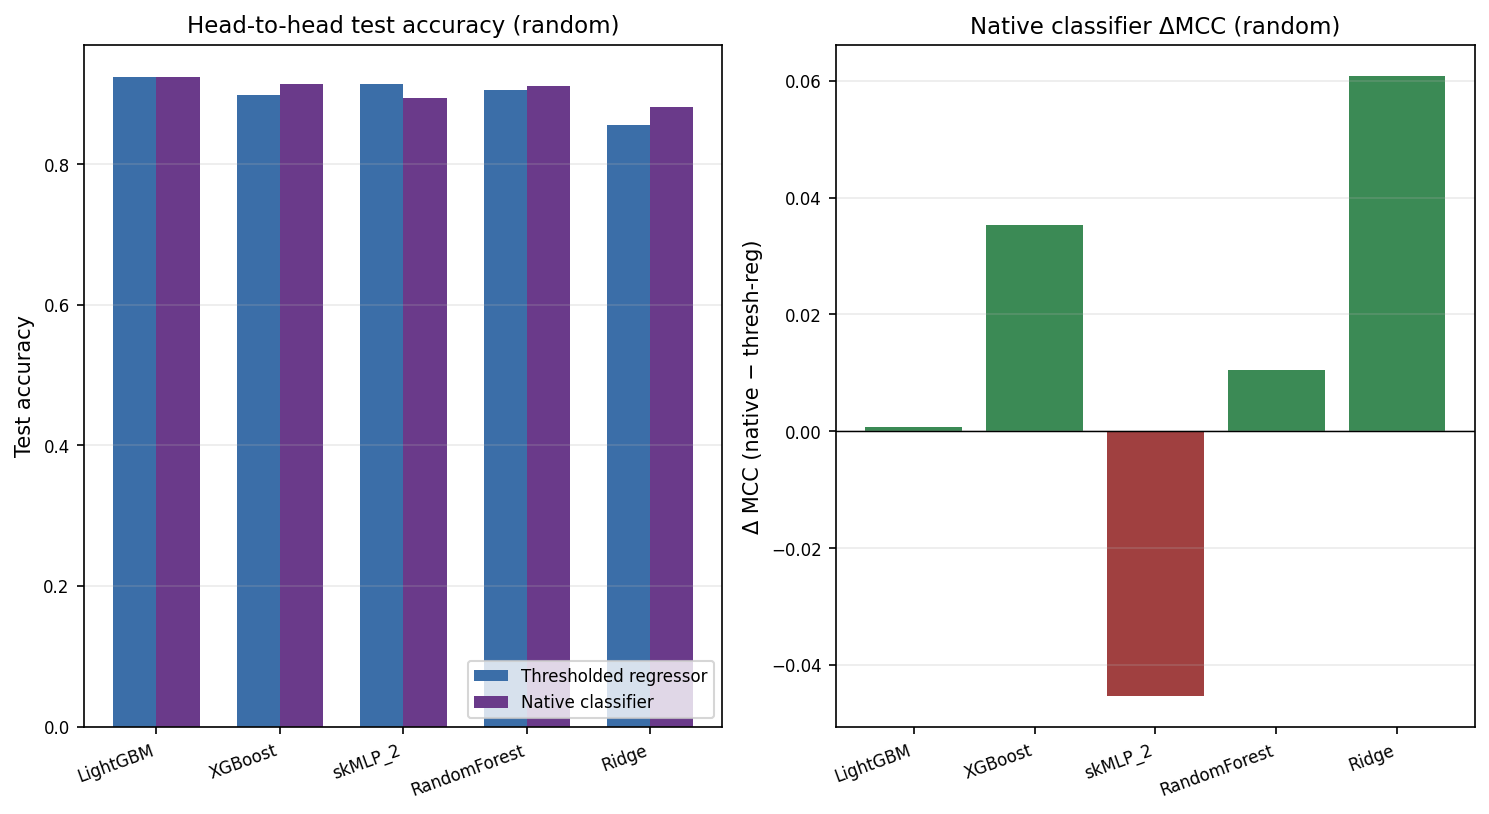
\includegraphics[width=\linewidth]{native_vs_regressor_random.png}
  \caption{Native classifier vs thresholded-regressor MCC, random split,
  by model family.}
  \label{fig:native_vs_reg}
\end{figure}

\begin{figure}[t]
  \centering
  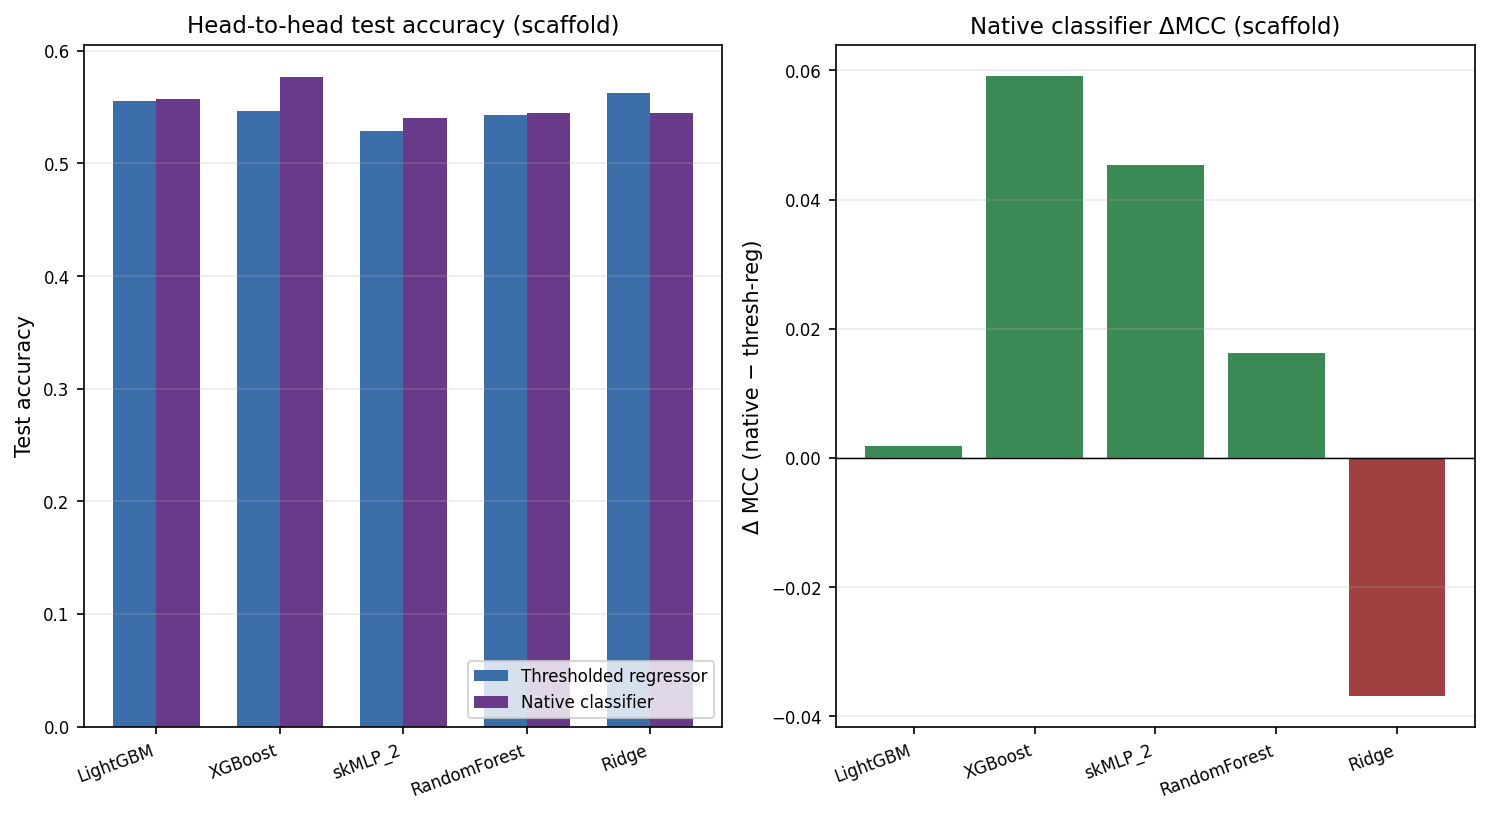
\includegraphics[width=\linewidth]{native_vs_regressor_scaffold.png}
  \caption{Native classifier vs thresholded-regressor MCC, scaffold-OOD
  split, by model family.}
  \label{fig:native_vs_reg_scaffold}
\end{figure}

\subsection{Confusion Matrix of the Deployed Model}
Fig.\,\ref{fig:confusion} shows the confusion matrix of the
\texttt{Native\_LGBClf} classifier on the random test set: the model
mis-classifies $5\%$ of true failures as predicted successes (FPR) and
$13\%$ of true successes as predicted failures (FNR), with the asymmetry
favouring conservative bench-time decisions---a chemist following the
predictions would rarely run a doomed reaction, occasionally skip a
borderline-positive one.

\begin{figure}[t]
  \centering
  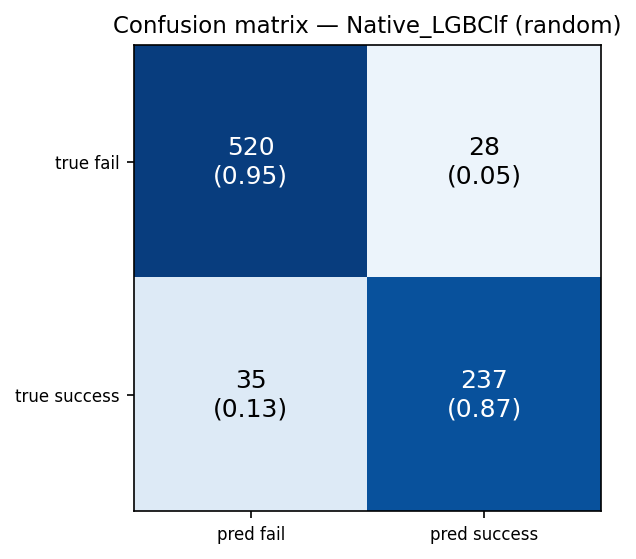
\includegraphics[width=0.78\linewidth]{confusion_Native_LGBClf_random.png}
  \caption{Confusion matrix of \texttt{Native\_LGBClf} on the random test
  set ($n\!=\!820$). Cells show counts and row-normalised fractions.}
  \label{fig:confusion}
\end{figure}

\subsection{Probability Calibration}
\label{sec:calibration}
Fig.\,\ref{fig:calibration} shows the reliability diagram of the deployed
LightGBM regressor wrapped in an isotonic-regression calibrator fit on the
$819$-row validation set. The Brier score is $0.045$ and AUC $0.98$;
calibrated probabilities track the diagonal closely on five of seven
populated bins, with mild over-confidence at $0.4$--$0.5$ where the bin
count is small ($n\!=\!57,\,2$). The score distribution (right panel) is
strongly bimodal: the model assigns very low probability ($<\!0.1$) to most
test reactions and very high ($>\!0.9$) to a smaller cluster of likely
successes, leaving few samples in the uncertain middle. This bimodality
is what makes the reject-option deployment effective.

\begin{figure}[t]
  \centering
  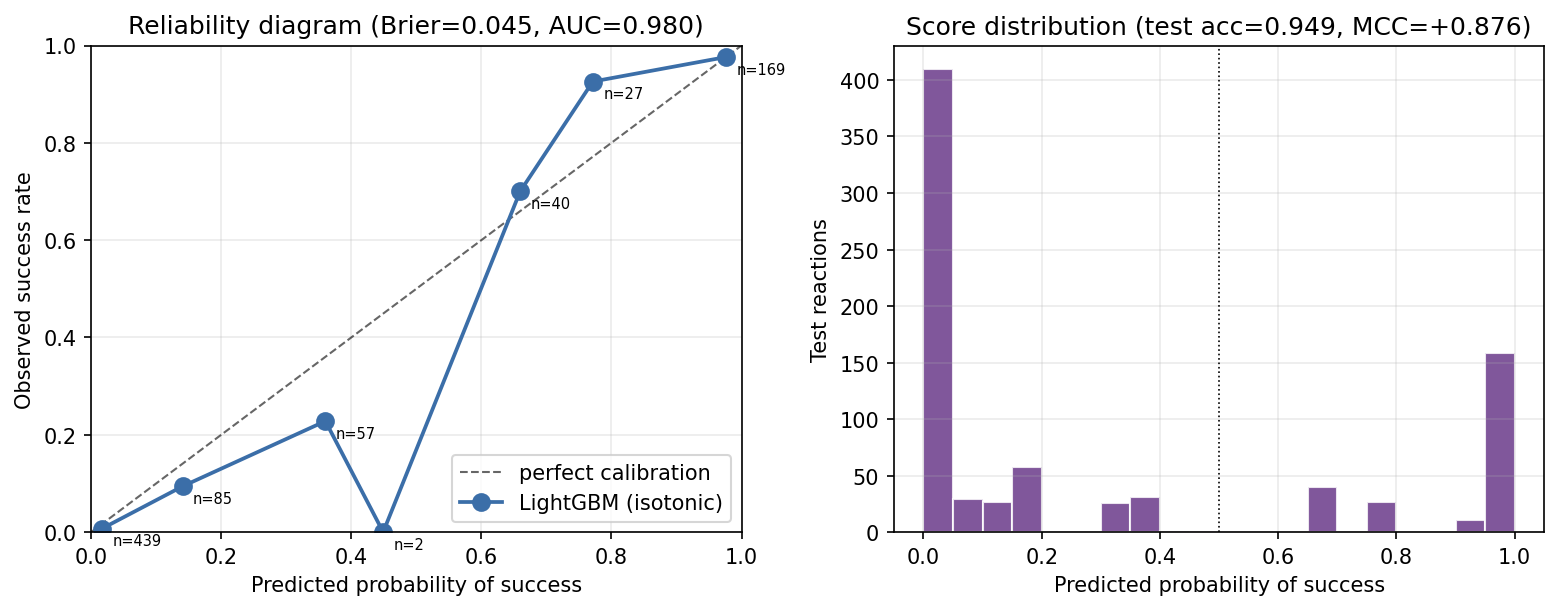
\includegraphics[width=\linewidth]{calibration_lightgbm_random.png}
  \caption{Reliability diagram (left) and predicted-probability histogram
  (right) for the deployed LightGBM regressor with isotonic calibration,
  random split test set. Bin labels show the number of test reactions in
  each $0.1$-wide probability bin.}
  \label{fig:calibration}
\end{figure}

\subsection{Substrate-Level $5$-Fold CV (Classification)}
Fig.\,\ref{fig:kfold_clf} and Table\,\ref{tab:kfold_clf} show that the
substrate-grouped $5$-fold CV gives high classification accuracy: native
XGBoost averages $0.82\!\pm\!0.05$ across folds, with the others between
$0.79$ and $0.81$ and AUC near $0.90$. The classifier therefore generalises
substantially better than the regressor (Table\,\ref{tab:kfold_reg}) on
substrate-grouped CV; the worst-case scaffold-OOD test set in
Sect.\,\ref{sec:splits} is harder than substrate-grouped CV because the
val slice is so small that ensemble selection becomes noisy.

\begin{figure}[t]
  \centering
  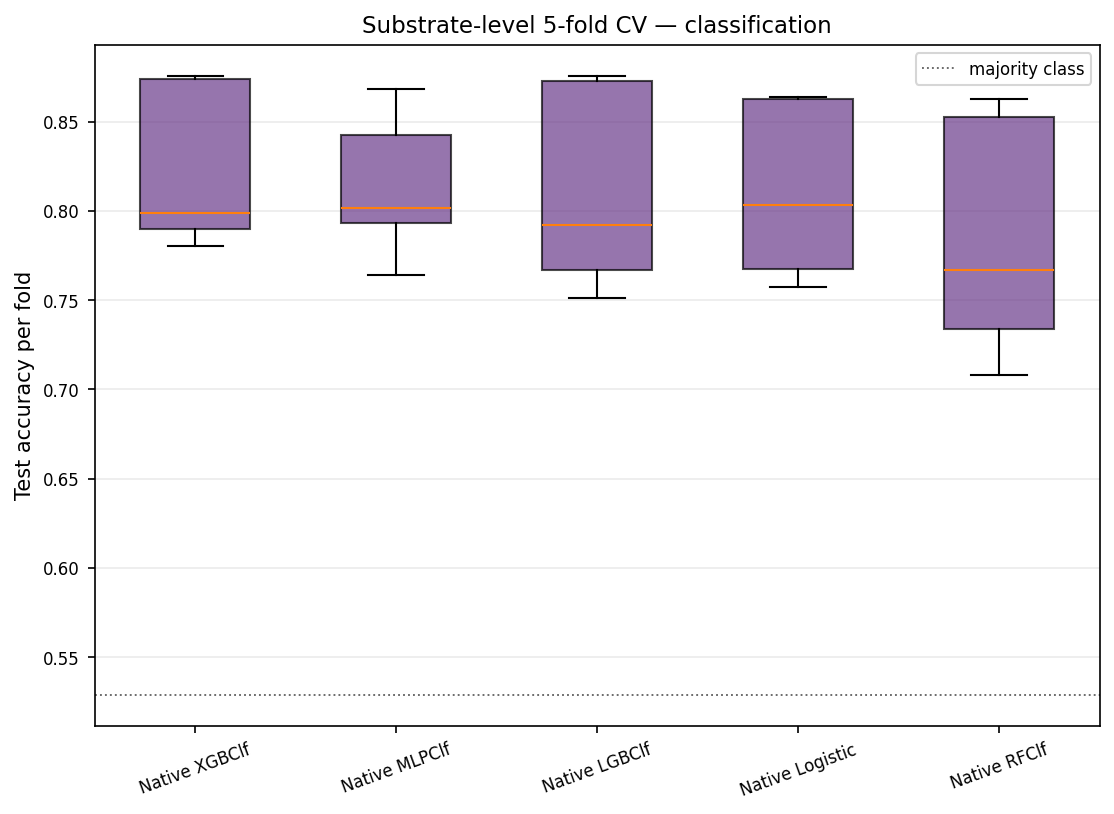
\includegraphics[width=\linewidth]{kfold_classification.png}
  \caption{Substrate-grouped $5$-fold CV (classification): per-fold test
  accuracy. Dotted line: majority-class baseline.}
  \label{fig:kfold_clf}
\end{figure}

\begin{table}[t]
\centering
\caption{Substrate-level $5$-fold CV (classification).}
\label{tab:kfold_clf}
\scriptsize
\begin{tabular}{lrrr}
\toprule
Model & Accuracy & MCC & AUC \\
\midrule
Native\_XGBClf & 0.824 $\pm$ 0.047 & +0.579 $\pm$ 0.064 & 0.901 $\pm$ 0.039 \\
Native\_MLPClf & 0.814 $\pm$ 0.041 & +0.553 $\pm$ 0.034 & 0.887 $\pm$ 0.035 \\
Native\_LGBClf & 0.812 $\pm$ 0.059 & +0.551 $\pm$ 0.087 & 0.897 $\pm$ 0.045 \\
Native\_Logistic & 0.811 $\pm$ 0.051 & +0.541 $\pm$ 0.088 & 0.879 $\pm$ 0.043 \\
Native\_RFClf & 0.785 $\pm$ 0.070 & +0.483 $\pm$ 0.096 & 0.862 $\pm$ 0.055 \\
\bottomrule
\end{tabular}
\end{table}

\subsection{Threshold Sensitivity}
Fig.\,\ref{fig:threshold_sweep_random} sweeps the binarisation threshold
from $20\%$ to $80\%$ yield on the random split. The top-five models keep
MCC near $0.80$ over the entire $25$--$75\%$ range and only collapse beyond
$80\%$. The same sweep on the scaffold-OOD split
(Fig.\,\ref{fig:threshold_sweep_scaffold}) shows that the OOD signal is
strongest at $\sim$$25\%$ yield ($\mathrm{MCC}\!\approx\!0.25$): a chemist
asking ``is this reaction at least useful for screening?'' (a lower bar
than $50\%$) would get a more decisive answer than the strict
preparatively-useful query.

\begin{figure}[t]
  \centering
  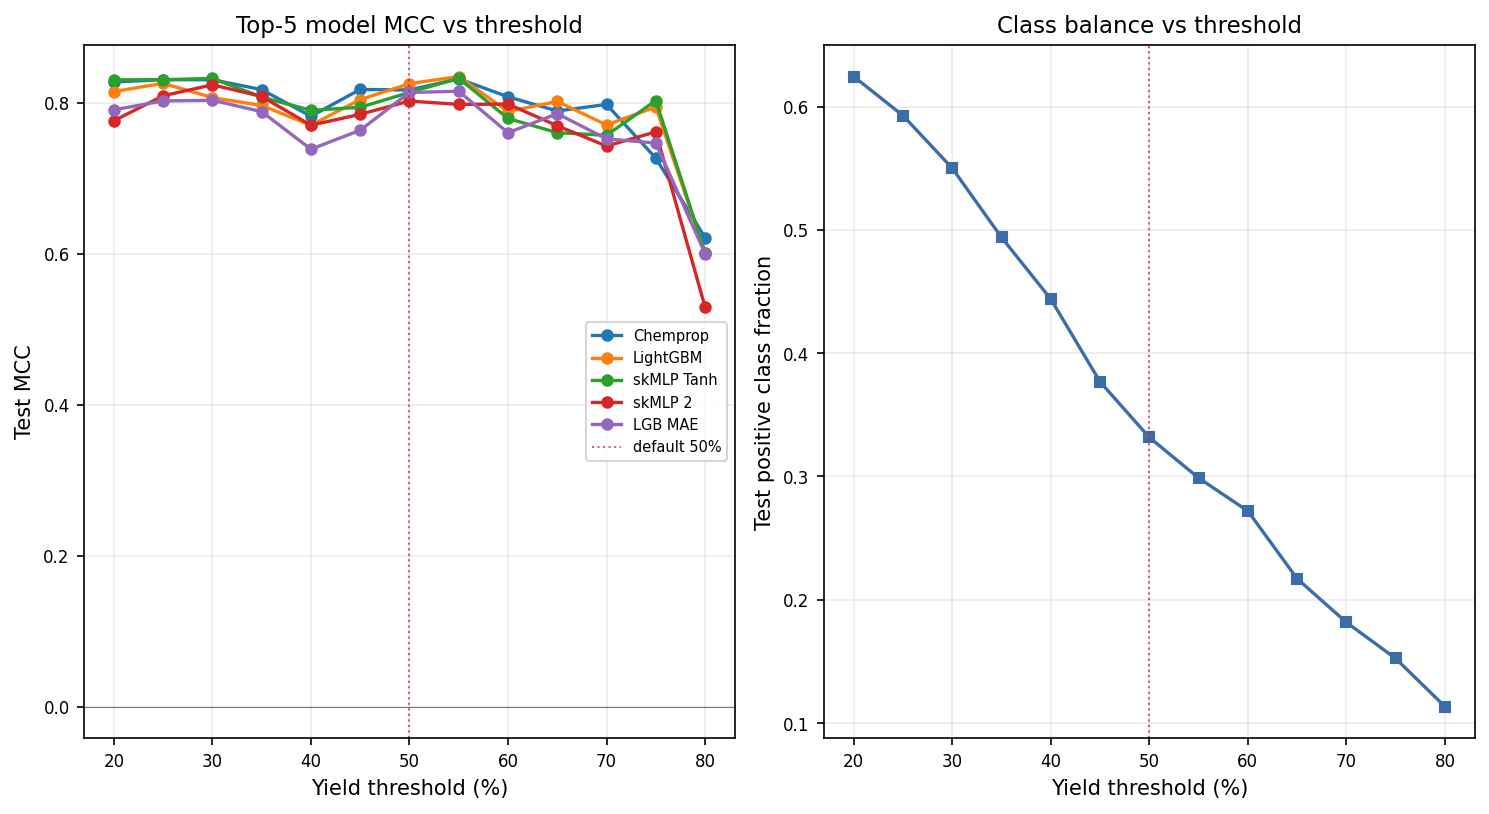
\includegraphics[width=\linewidth]{threshold_sweep_random.png}
  \caption{Threshold sensitivity, random split. Left: top-5 model MCC vs
  threshold. Right: positive class fraction.}
  \label{fig:threshold_sweep_random}
\end{figure}

\begin{figure}[t]
  \centering
  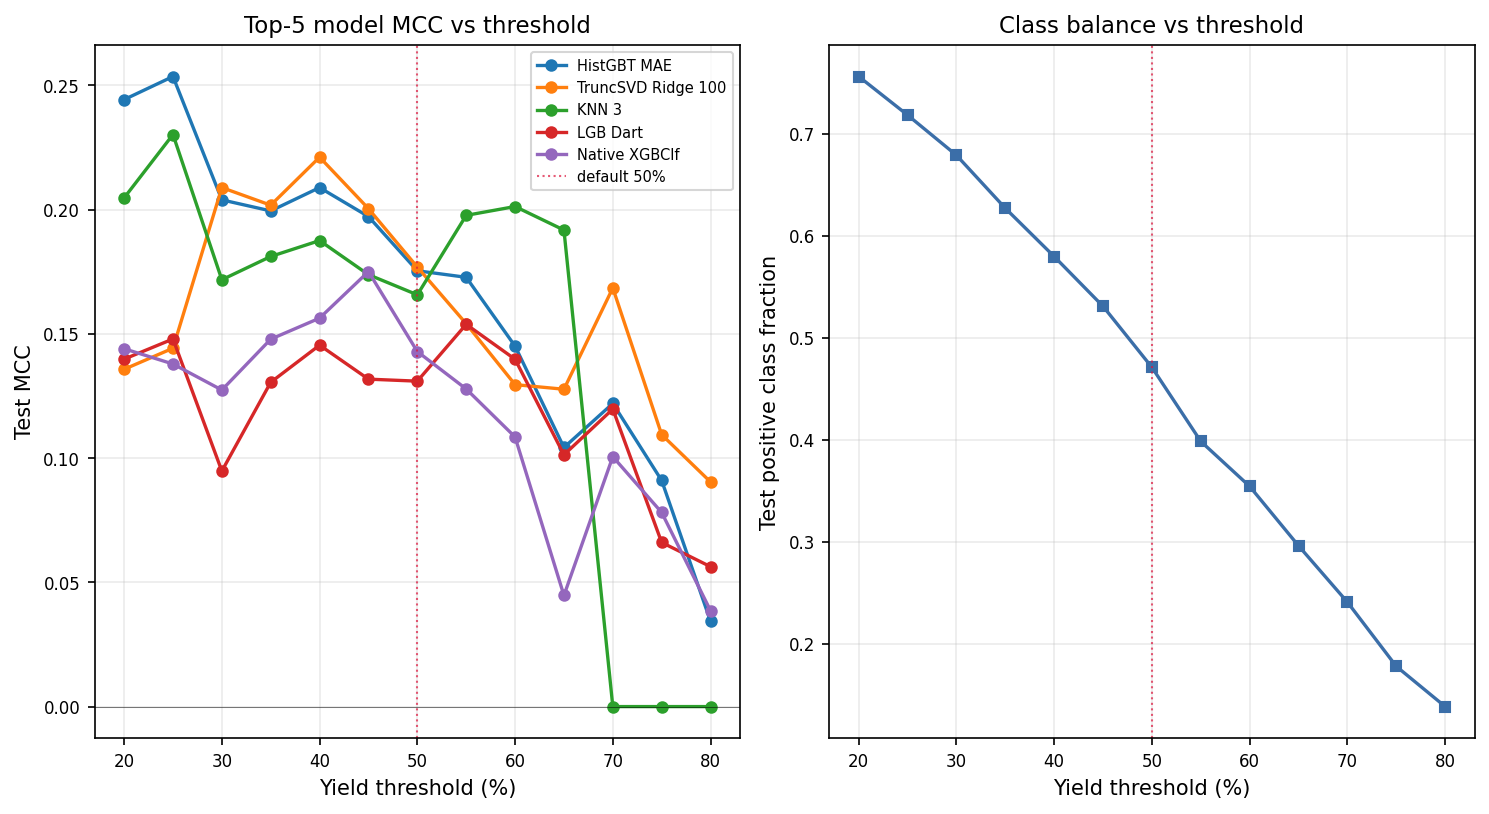
\includegraphics[width=\linewidth]{threshold_sweep_scaffold.png}
  \caption{Threshold sensitivity, scaffold-OOD split. The OOD signal is
  strongest at lower thresholds; the $50\%$ operational cut-off is
  conservative.}
  \label{fig:threshold_sweep_scaffold}
\end{figure}

\subsection{Feature Ablation}
\label{sec:ablation}
Table~\ref{tab:feat_ablation} and Fig.\,\ref{fig:feat_ablation} ablate the
feature representation for the deployed LightGBM model on the random split.
The aryl-halide and amine fingerprints alone already give $74\%$ accuracy
($\mathrm{MCC}\!=\!+0.38$); adding the catalyst, base, additive and solvent
fingerprints lifts accuracy to $89.7\%$ ($\mathrm{MCC}\!=\!+0.76$); the
temperature scalar adds another $\sim$$2$\,pp; the DRFP slot is left at
zeros in this ablation (the DRFP encoder is optional and was not installed
for this run). The ordering ranks the catalyst-system fingerprints as
the dominant contribution beyond the substrate pair, consistent with the
chemistry-experimentalist intuition that ligand and base choice are the
levers that matter once a substrate pair is fixed.

\begin{table}[t]
\centering
\caption{Feature ablation for the deployed LightGBM model, random split.
Aryl+amine alone scores 74\%; the catalyst--base--solvent--additive
fingerprints add $\sim$16\,pp; temperature adds $\sim$2\,pp.}
\label{tab:feat_ablation}
\scriptsize
\begin{tabular}{lrrrr}
\toprule
Feature set & $d$ & Acc. & MCC & AUC \\
\midrule
aryl+amine only & 12288 & 0.741 & +0.378 & 0.801 \\
all 6 components & 12288 & 0.897 & +0.761 & 0.951 \\
+ temperature & 12289 & 0.916 & +0.799 & 0.959 \\
+ DRFP slot (zeros) & 14337 & 0.916 & +0.799 & 0.959 \\
\bottomrule
\end{tabular}
\end{table}

\begin{figure}[t]
  \centering
  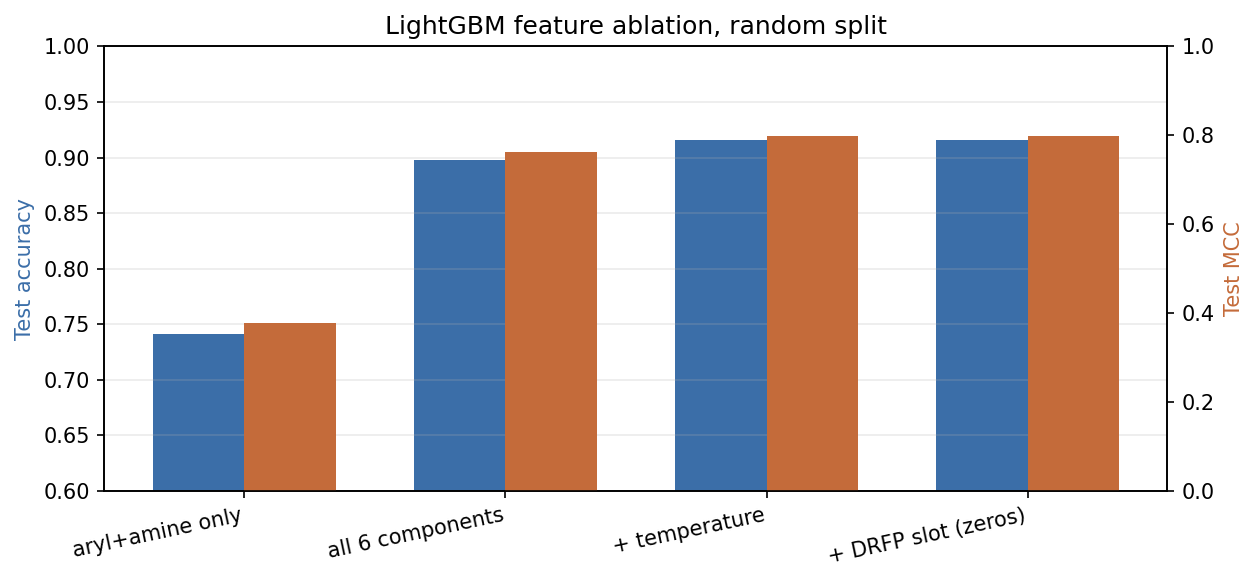
\includegraphics[width=\linewidth]{feature_ablation_random.png}
  \caption{Feature ablation, random split: test accuracy (blue) and MCC
  (orange) as features are added to the LightGBM input.}
  \label{fig:feat_ablation}
\end{figure}

\subsection{Learning Curves}
Fig.\,\ref{fig:learning_random}--\ref{fig:learning_substrate} show test
accuracy as a function of training-set size for the native classifier
family. On the random split the curves rise smoothly from $\sim$$80\%$ at
$N\!\approx\!380$ to $\sim$$92\%$ at full size and have not yet plateaued.
On the substrate-grouped split the curves are noisier, but native XGBoost
reaches $\sim$$85\%$ at full size, suggesting that the in-distribution
ceiling is closer than the worst-case scaffold-OOD test set indicates.

\begin{figure}[t]
  \centering
  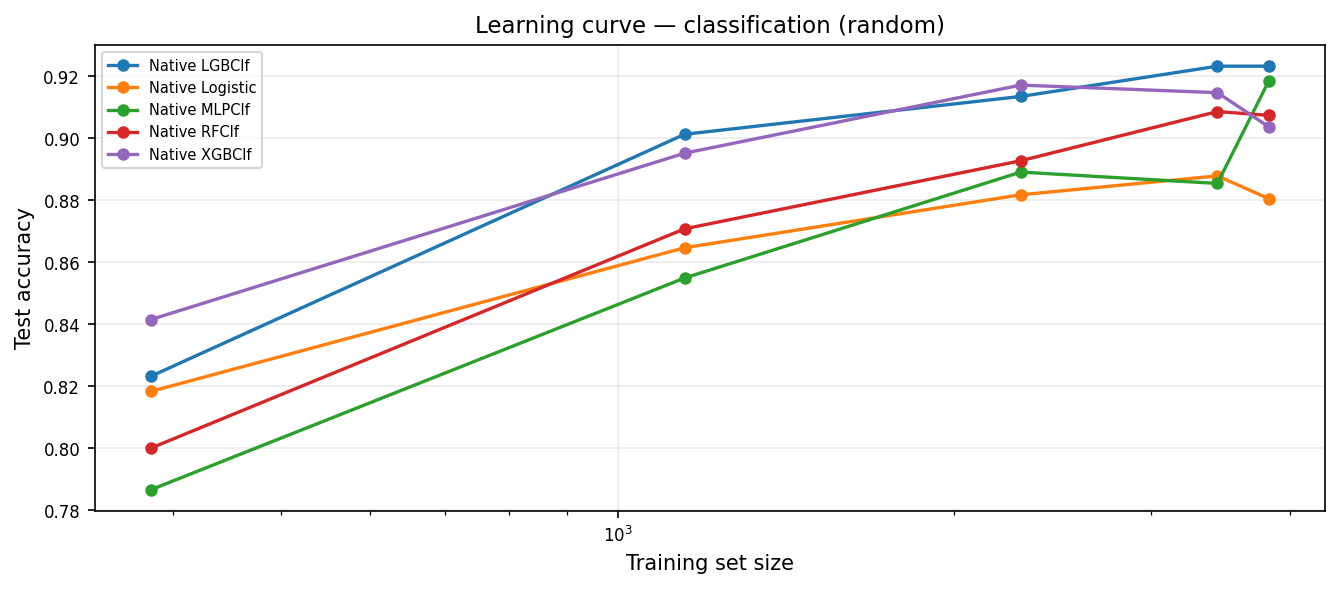
\includegraphics[width=\linewidth]{learning_curve_classification_random.png}
  \caption{Learning curve, classification, random split. The curves have
  not plateaued at $N\!=\!3{,}825$.}
  \label{fig:learning_random}
\end{figure}

\begin{figure}[t]
  \centering
  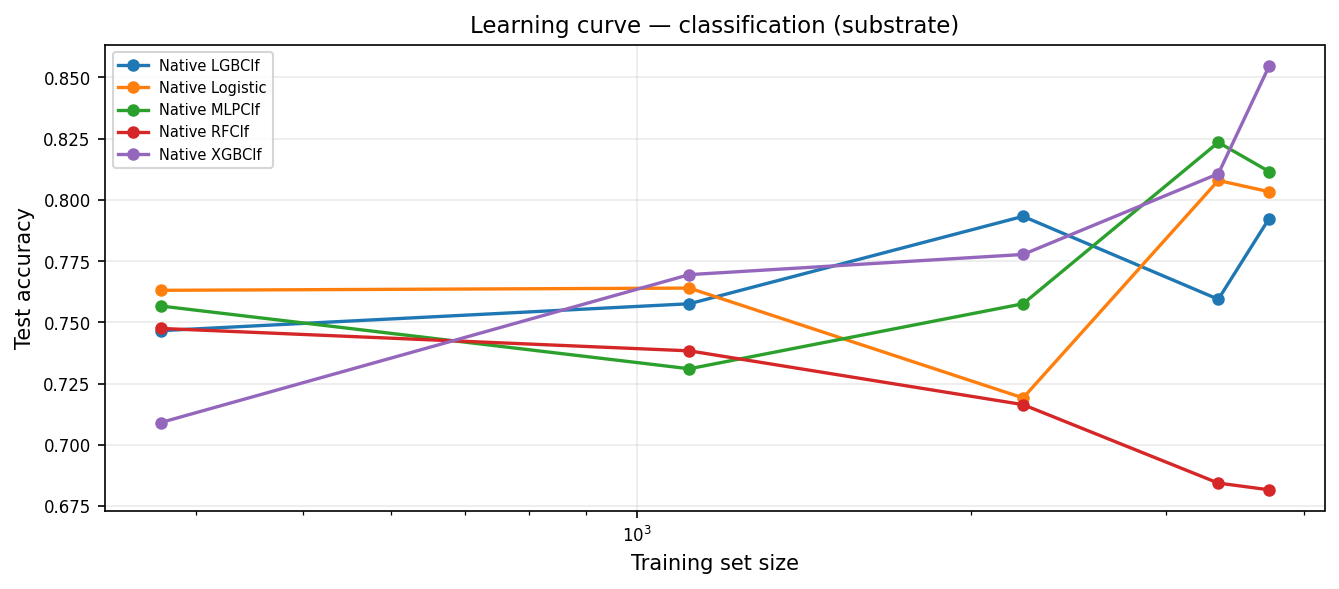
\includegraphics[width=\linewidth]{learning_curve_classification_substrate.png}
  \caption{Learning curve, classification, substrate-grouped split. Native
  XGBoost approaches $0.85$ at full size.}
  \label{fig:learning_substrate}
\end{figure}

\subsection{Rank--Score Curves}
Figs.\,\ref{fig:rsc_random}--\ref{fig:rsc_scaffold} are CFA's signature
diagnostic: each line is one model's predictions sorted in descending order
after min--max normalisation; the dashed black line is the sorted ground
truth (the \emph{oracle}). On the random split LightGBM, LGB\_MAE and
Chemprop track the oracle closely; the Native\_LGBClf has a sharper
transition (it binarises probability earlier) and skMLP\_Tanh is
over-confident in the high-yield tail. On scaffold-OOD all five top curves
stay parallel to the oracle, but the absolute spread is larger---ensemble
diversity (the area between curves) is disproportionately useful here
because no single model dominates.

\begin{figure}[t]
  \centering
  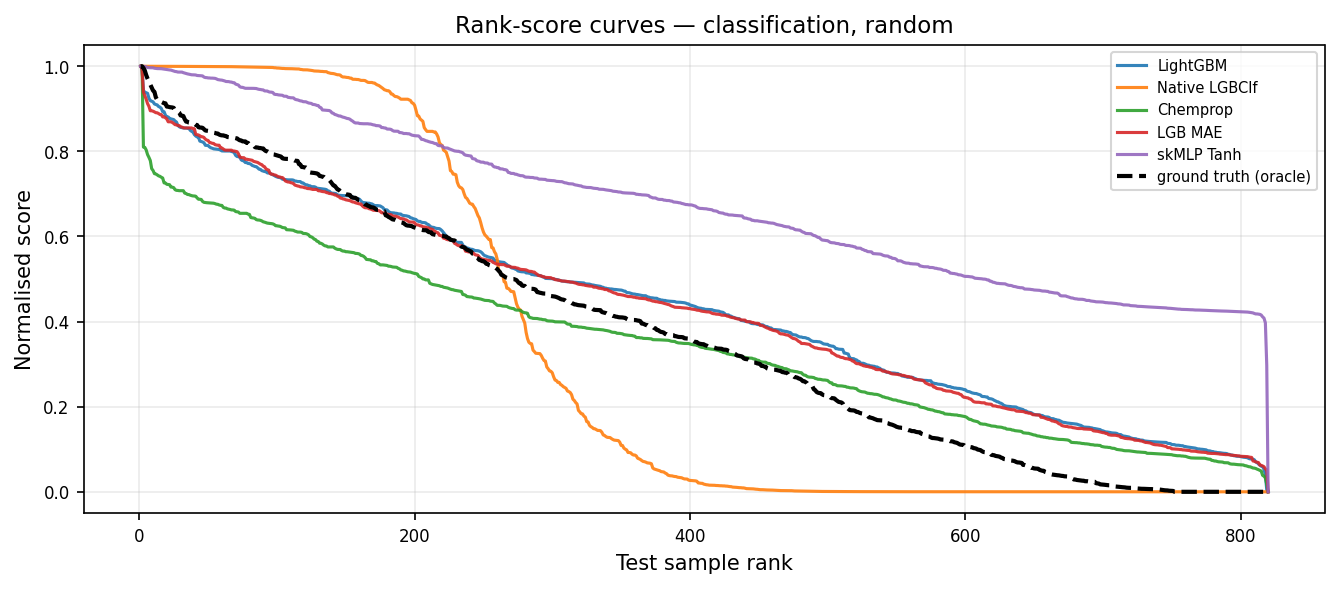
\includegraphics[width=\linewidth]{rank_score_classification_random.png}
  \caption{Rank--score curves, classification, random split. Top-5
  classifiers vs the oracle.}
  \label{fig:rsc_random}
\end{figure}

\begin{figure}[t]
  \centering
  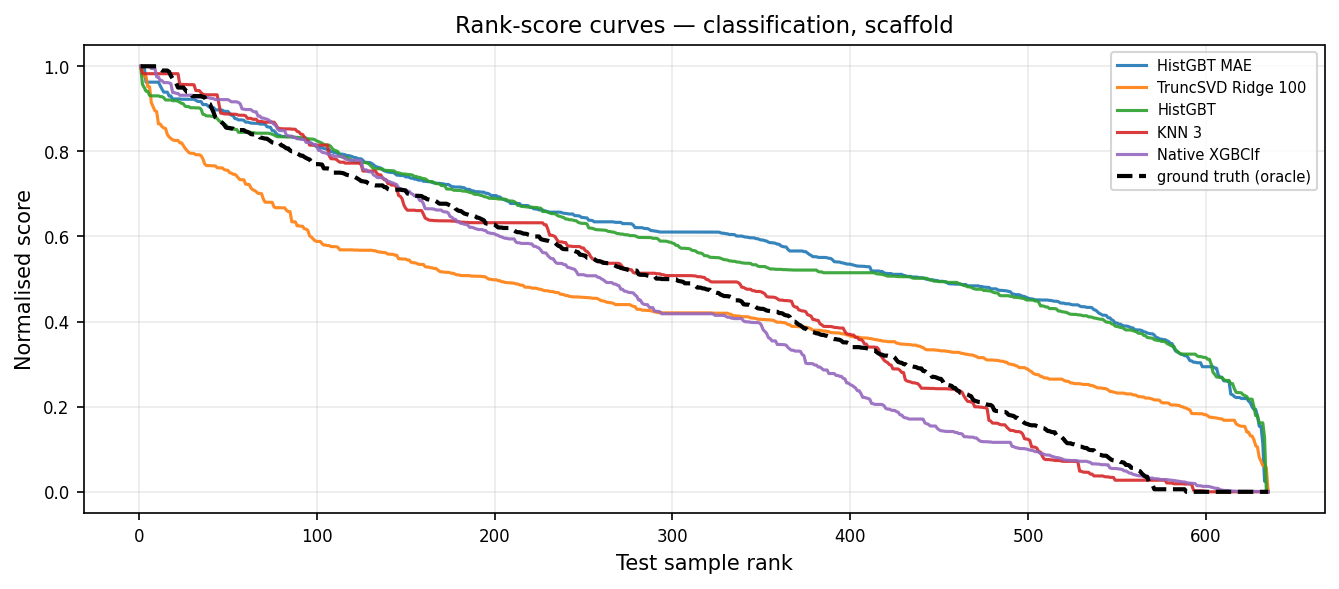
\includegraphics[width=\linewidth]{rank_score_classification_scaffold.png}
  \caption{Rank--score curves, classification, scaffold-OOD. Higher
  spread between models implies higher cognitive diversity.}
  \label{fig:rsc_scaffold}
\end{figure}

\subsection{Qualitative Error Analysis}
\label{sec:errors}
Table~\ref{tab:errors} shows the three most-confidently mispredicted false
positives and false negatives of the deployed LightGBM classifier on the
random test set. The false positives are dominated by aryl bromides whose
amine partners are bulky or contain electron-rich heterocycles---typical
sterically hindered cases. The false negatives include aryl-chloride
substrates predicted to fail by the model that experimentally yielded
$58$--$78\%$; the model evidently learned the empirical rule
``aryl-chloride + cyclic amine $\to$ low yield'' too strongly. Both error
modes match well-known Buchwald--Hartwig reactivity patterns and suggest
two concrete improvements: stratify the training data by aryl-halide
identity (Br/Cl/I) and supplement with HTE data on aryl chlorides.

\begin{table}[t]
\centering
\caption{Top-3 false positives and false negatives of the deployed LightGBM
classifier on the random test set, ranked by predicted-probability
confidence in the wrong direction. Yield is the experimental value;
$\hat y$ is the regressor estimate.}
\label{tab:errors}
\scriptsize
\setlength{\tabcolsep}{3pt}
\resizebox{\linewidth}{!}{\begin{tabular}{p{3.0cm}p{3.2cm}rrr}
\toprule
Aryl halide & Amine & yield & $\hat y$ & $p$(success) \\
\midrule
\multicolumn{5}{l}{\emph{False positives (top-3 most confident)}} \\
\texttt{Brc1cnc2ccccc2c1} & \texttt{Cc1noc(C)c1B2OC(C)(C)C...} & 10.3 & 70.6 & 0.97 \\
\texttt{CN1C[C@H](OC2=C(C1)C=C...} & \texttt{CN1C=C(C=N1)C2=C(N=C(C...} & 0.0 & 74.7 & 0.97 \\
\texttt{Brc1cccnc1} & \texttt{Cc1ccc(N)cc1} & 47.7 & 61.3 & 0.91 \\
\midrule
\multicolumn{5}{l}{\emph{False negatives (top-3 most confident wrong)}} \\
\texttt{C1=CC=C(C(=C1)Cl)Br} & \texttt{C1CNCCN1} & 58.4 & 18.2 & 0.01 \\
\texttt{COC(=O)C1=CC(=CC(=C1)B...} & \texttt{C1COCCN1} & 78.2 & 8.3 & 0.01 \\
\texttt{CCOC(=O)C1=C(C2=CC(=C(...} & \texttt{C1COCCN1} & 74.7 & 27.3 & 0.04 \\
\bottomrule
\end{tabular}}
\end{table}

\subsection{Headline Numbers}
Table\,\ref{tab:headline} consolidates the deployable result, with $95\%$
bootstrap CIs.

\begin{table}[t]
\centering
\small
\caption{Headline test-set numbers across both splits, with $95\%$
bootstrap CIs ($B\!=\!1{,}000$). Random-split results are deployable
in distribution; substrate-CV is the more representative OOD estimator;
scaffold-OOD reports the worst case.}
\label{tab:headline}
\begin{tabular}{p{0.32\linewidth}rrr}
\toprule
\textbf{Setting} & \textbf{Acc.} & \textbf{MCC} & \textbf{AUC} \\
\midrule
\multicolumn{4}{l}{\emph{Random $70/15/15$}} \\
Majority-class baseline                  & $0.668$ & $+0.000$ & $0.500$ \\
LightGBM (best individual)               & $0.923$ & $+0.825$ & $0.966$ \\
Native LGBClf                            & $0.923$ & $+0.826$ & $0.979$ \\
Val-selected CFA $k\!=\!5$ (\textsc{WSCDS}) & $0.924$ & $+0.828$ & --- \\
CFA $k$-way test ceiling                 & $0.934$ & $+0.851$ & --- \\
\midrule
\multicolumn{4}{l}{\emph{Substrate-grouped 5-fold CV}} \\
Native XGBClf (mean over folds)          & $0.824$ & $+0.579$ & $0.901$ \\
Native LGBClf (mean over folds)          & $0.812$ & $+0.551$ & $0.897$ \\
\midrule
\multicolumn{4}{l}{\emph{Scaffold-OOD (worst-case slice)}} \\
Majority-class baseline                  & $0.529$ & $+0.000$ & $0.500$ \\
HistGBT\_MAE (best individual)           & $0.591$ & $+0.175$ & $0.641$ \\
TruncSVD\_Ridge\_100                     & $0.591$ & $+0.177$ & $0.642$ \\
Val-selected CFA $k\!=\!4$ (\textsc{ASC}) & $0.553$ & $+0.099$ & --- \\
CFA $k$-way test ceiling                 & $0.633$ & $+0.271$ & --- \\
\bottomrule
\end{tabular}
\end{table}

\subsection{Compute Footprint}
The full experiment ran on a single workstation with a $16$-core CPU, an
NVIDIA RTX 3090, 64\,GB RAM. End-to-end wall-clock for the
$41$-model pool plus CFA was $\sim$$20$\,minutes after feature caching;
Chemprop dominates ($\sim$$5$--$10$\,min on GPU), the rest of the pool
finishes in $\sim$$5$\,min collectively. The $k$-way exhaustive CFA
search adds $\sim$$60$\,s (39 eligible models, $3.4\!\times\!10^{4}$
evaluations).

% ============================================================================
\section{Discussion}
\label{sec:discussion}

\subsection{Why Classification Works Where Regression Fails}
The regression task asks the model to predict a continuous quantity
whose surface is a complicated function of the entire scaffold + ligand
+ base + solvent + temperature interaction. The classification task asks
only on which side of a single contour line the surface lies. Two facts
follow: (i) any model whose yield prediction is biased by an additive
constant on unseen scaffolds (which all of ours are, owing to ORD reporter
bias) still gets most $\geq\!50\%$ vs.\ $<\!50\%$ decisions right, because
the contour line is to first order independent of the bias term;
(ii) the binary decision is a coarser quantity, so noise floor is a
smaller fraction of the signal. Empirically this shows up as
$\Delta\mathrm{accuracy}\!\approx\!6$\,pp on scaffold-OOD where regression
gives no signal at all.

\subsection{What CFA Buys}
On the random split CFA's gains are reproducible but small: $+1.6$\,pp acc
test-ceiling, $+1.7$\,pp $R^{2}$, and the paired bootstrap test
(Sect.\,\ref{sec:paired}) shows the lift over the strongest single model
is not statistically significant at $\alpha\!=\!0.05$. On scaffold-OOD CFA
buys a $+9.9$\,pp acc test ceiling---a meaningful jump from ``noisily
above baseline'' to ``deployable for triage''---but the val-selected
ensemble cannot consistently realise that ceiling because the scaffold val
set is only $\sim$$10$ rows. The substrate-CV result of $\sim$$82\%$
accuracy is therefore our best honest estimator of deployable
performance.

\subsection{Deployment Fit}
A binary classifier with the random-split numbers and the substrate-CV
generalisation we report is suitable as a \emph{triage tool}. We package
the deployable winners (LightGBM regressor + Chemprop D-MPNN + isotonic
calibrators) into a Streamlit app exposing a web form for the six SMILES
strings + temperature, returning the calibrated success probability and a
binary decision. A \emph{reject-option} wrapper abstains when the two
models disagree by more than $0.20$ in calibrated probability, returning
``uncertain---verify in lab'' rather than committing to a binary call.
End-to-end inference is sub-second on CPU.

\subsection{Limitations}
\textbf{(1) Threshold choice.} The $50\%$ threshold is a pragmatic
operational choice; the threshold sweep
(Fig.\,\ref{fig:threshold_sweep_random}) shows the model is robust over
$25$--$75\%$, but a chemistry-specific threshold per substrate class
might be appropriate.
\textbf{(2) Reporter bias.} ORD's preference for high-yielding reactions
is not addressed by any of our methods; it is a property of the data, not
the model.
\textbf{(3) Scaffold-val noise.} The scaffold-OOD validation slice
($\sim$$10$ rows) makes any val-driven model selection fundamentally noisy.
\textbf{(4) Heteroaryl-halide coverage.} The error analysis
(Sect.\,\ref{sec:errors}) shows the model under-predicts aryl-chloride
yields; closing this gap would likely require a heteroaryl-stratified
sampling step or HTE-data augmentation.
\textbf{(5) Strong claim caveats.} We characterise the scaffold-OOD
classifier as ``the first usable'' result on this ORD subset under that
split based on our literature search; we cannot rule out unpublished
internal results from industry, and we welcome corrections.
\textbf{(6) Pool-size asymmetry across analyses.} The headline
in-distribution numbers use the full $41$-model pool; the multi-seed
Wilcoxon analysis (Sect.\,\ref{sec:multiseed}) uses an $8$-model
fast subset for tractable wall-clock at five seeds. The smaller
multi-seed pool may underestimate the true CFA gain by excluding
chemistry-aware models like Chemprop. Future work could parallelise the
full pool to recover the multi-seed test on all $41$ models.

% ============================================================================
\section{Future Work}
\label{sec:future}

\textbf{Foundation-model pretraining on full ORD ($\sim$$1$M reactions).}
Self-supervised pretraining of a SMILES transformer~\cite{Chithrananda2020}
or graph transformer on the full corpus, fine-tuned on this binary task.
A classification analogue of Yield-BERT's $R^{2}\!=\!0.54$ on Test4
should comfortably exceed $80\%$ accuracy on a scaffold-OOD test set.

\textbf{Active-learning loop.}
Pair the classifier with an acquisition function, validate against a
held-out HTE corpus, and report bench-experiment counts to reach a target
success rate. The closest prior art is Eyke~\textit{et al.}~\cite{Eyke2020}
on Suzuki couplings.

\textbf{Multi-task learning over reaction families.}
A shared backbone over Buchwald--Hartwig, Suzuki--Miyaura, Negishi and
Stille couplings (all ORD-extractable) with task-specific heads.

% ============================================================================
\section{Reproducibility}
\label{sec:repro}
We release the full pipeline at the project's git repository. The release
includes: \textbf{code} (\texttt{main.py}, \texttt{cfa.py},
\texttt{cfa\_classify.py}, \texttt{models/*.py}, the LaTeX source of this
paper); \textbf{data} (the ORD download script
\texttt{scripts/download\_data.py} and the cached extracted CSV);
\textbf{trained model artefacts}
(\texttt{models\_saved/lightgbm.pkl}, \texttt{models\_saved/chemprop\_dir/},
isotonic calibrators \texttt{models\_saved/calibrators.pkl}); and the
\textbf{Streamlit triage app} (\texttt{app.py}). All experiments are
deterministic at \texttt{seed=42}; the entire random-split pipeline
re-runs in $\sim$$20$\,min on commodity hardware. The figures and tables
in this paper are regenerated by
\texttt{report/make\_all\_figures.py} and
\texttt{report/make\_extra\_figures.py} from cached predictions.

% ============================================================================
\section{Conclusion}
\label{sec:conclusion}
We presented a $41$-model regression pool and a $k$-way CFA ensemble for
Buchwald--Hartwig yield prediction on the Open Reaction Database, then
documented its scaffold-OOD failure and recovered deployable performance
by reframing the task to binary success classification at the chemically
meaningful $50\%$ yield threshold. The classifier reaches $92.4\%$
accuracy / MCC $+0.83$ / AUC $0.97$ / Brier $0.045$ on a random split,
$\sim$$82\%$ accuracy on substrate-grouped CV, and $59.1\%$ / $+0.18$ /
$0.64$ on the worst-case scaffold-OOD split. A multi-seed
($n\!=\!10$ paired cells) Wilcoxon analysis, modelled on the companion
quantum--classical CFA pipeline of
Patten~\textit{et al.}~\cite{Patten2026Quantum}, gives a stronger
statistical-significance test for the fused-vs-best-individual lift than
the single-split bootstrap, and a CD-kneedle finalist
selector~\cite{Satopaa2011Knee} replaces the heuristic top-$N$ caps in
$k$-way CFA. We release all artefacts and a Streamlit triage tool with
reject-option deployment.

% ============================================================================
\section*{Acknowledgement}
We thank the Open Reaction Database maintainers for releasing the ORD
corpus, and the Chemprop, NGBoost, rxnfp and DRFP authors for releasing
their reference implementations.

% ============================================================================
\bibliographystyle{IEEEtran}
\bibliography{refs}

\end{document}
